\documentclass[conference, compsoc]{IEEEtran}
\usepackage{graphicx}
\usepackage{array, float}
\usepackage[colorlinks=true]{hyperref}
\usepackage[style=numeric,backend=bibtex]{biblatex}
\graphicspath{ {./figures/} }
\addbibresource{refs.bib}

\begin{document}

\title{Dataset Distillation: A Data-Efficient Learning Framework}
\author{Swapnil Patel - 999728870 - \today}

\author{\IEEEauthorblockN{Swapnil Patel}
	\IEEEauthorblockA{
		University of Toronto\\
		swap.patel@mail.utoronto.ca\\
		\url{https://github.com/Swapnil949/ECE1512\_2024F\_ProjectRepo\_SwapnilPatel}
	}}

\maketitle

\begin{abstract}
\label{sec:abstract}
The entire project source can be found at: \href{https://github.com/Swapnil949/ECE1512_2024F_ProjectRepo_SwapnilPatel}{Github Repository}.

\end{abstract}

\section{Introduction}
\label{sec:intro}

Dataset Distillation is an emerging technique in machine learning designed to compress large datasets into smaller, synthetic datasets that retain the critical information needed to train neural networks effectively. This approach addresses the growing demand for computational efficiency by significantly reducing memory requirements and training times without compromising model performance. By distilling the essential features of a vast dataset, researchers can train models on a compact, representative subset, thus enabling rapid prototyping and exploration of deep learning architectures. As dataset sizes continue to expand, methods such as dataset distillation offer promising pathways for scalable and resource-efficient machine learning. \\

Dataset distillation has several applications such as \textit{Neural Architecture Search (NAS)}, \textit{Privacy Preservation}, \textit{Federated Learning}, \textit{Memory-efficient Continual Learning}, and \textit{Data sharing}.

\subsubsection*{Neural Architecture Search (NAS)}
In NAS, dataset distillation provides a compact proxy dataset that approximates the performance of training on a full-scale dataset \cite{white2023neuralarchitecturesearchinsights}. This enables faster and more resource-efficient model evaluation across architectures, allowing for rapid exploration and selection of optimal models without the computational expense of using the full dataset.

\subsubsection*{Privacy Preservation}
For privacy preservation, distilled datasets reduce exposure to sensitive information by retaining only essential features rather than raw, identifiable data \cite{dong2022privacyfreedoesdataset}. This allows machine learning models to be trained securely in privacy-sensitive domains (e.g., healthcare and finance) and enhances data sharing compliance in settings like federated learning.

\section{Dataset Distillation with Attention Matching}
The paper "DataDAM: Efficient Dataset Distillation with Attention Matching" \cite{sajedi2023datadamefficientdatasetdistillation} presents a novel dataset distillation approach aimed at reducing training dataset sizes while retaining essential information. The primary challenge addressed by the authors is the high computational cost associated with deep learning models when using full-sized datasets.

In this work, the authors generate a synthetic dataset by employing \texttt{Spatial Attention Mapping (SAM)} to capture attention maps from real and synthetic data across various layers within a family of randomly initialized neural networks. This approach alleviates the substantial memory demands typically encountered in state-of-the-art methods. The use of randomly initialized neural network instead of Pre-trained models also makes their solution more versatile and improves cross-architecture generalization results. 

Additionally, they introduce a \texttt{complementary loss} as a regularization technique to align the last-layer feature distributions between the real and synthetic datasets. Fig. \ref{fig:datadam_method} illustrates the novel methodology proposed by the authors.

% Privacy 

% neural Network search

\begin{figure}[H]
	\centering
	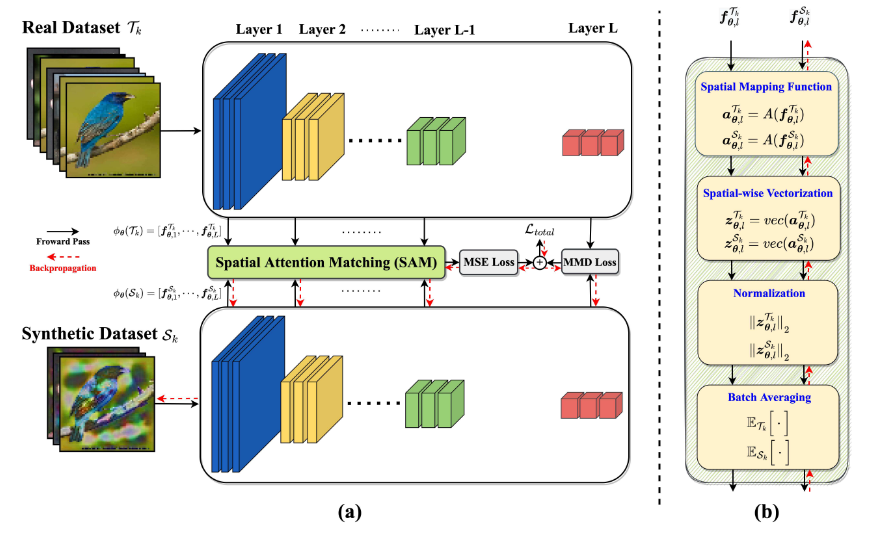
\includegraphics[width=0.48\textwidth]{datadam.png}
	\caption{DataDAM Method \cite{sajedi2023datadamefficientdatasetdistillation}}
	\label{fig:datadam_method}
\end{figure}

With this new method, authors are able to beat existing state-of-the-art solutions by improving performance by 6.5\% for CIFAR100 and 4.1\% for ImageNet-1k. They also achieve up to a 100x reduction in training costs for learning synthetic dataset.
 
\subsection{MNIST Dataset}
\begin{figure}[H]
	\centering
	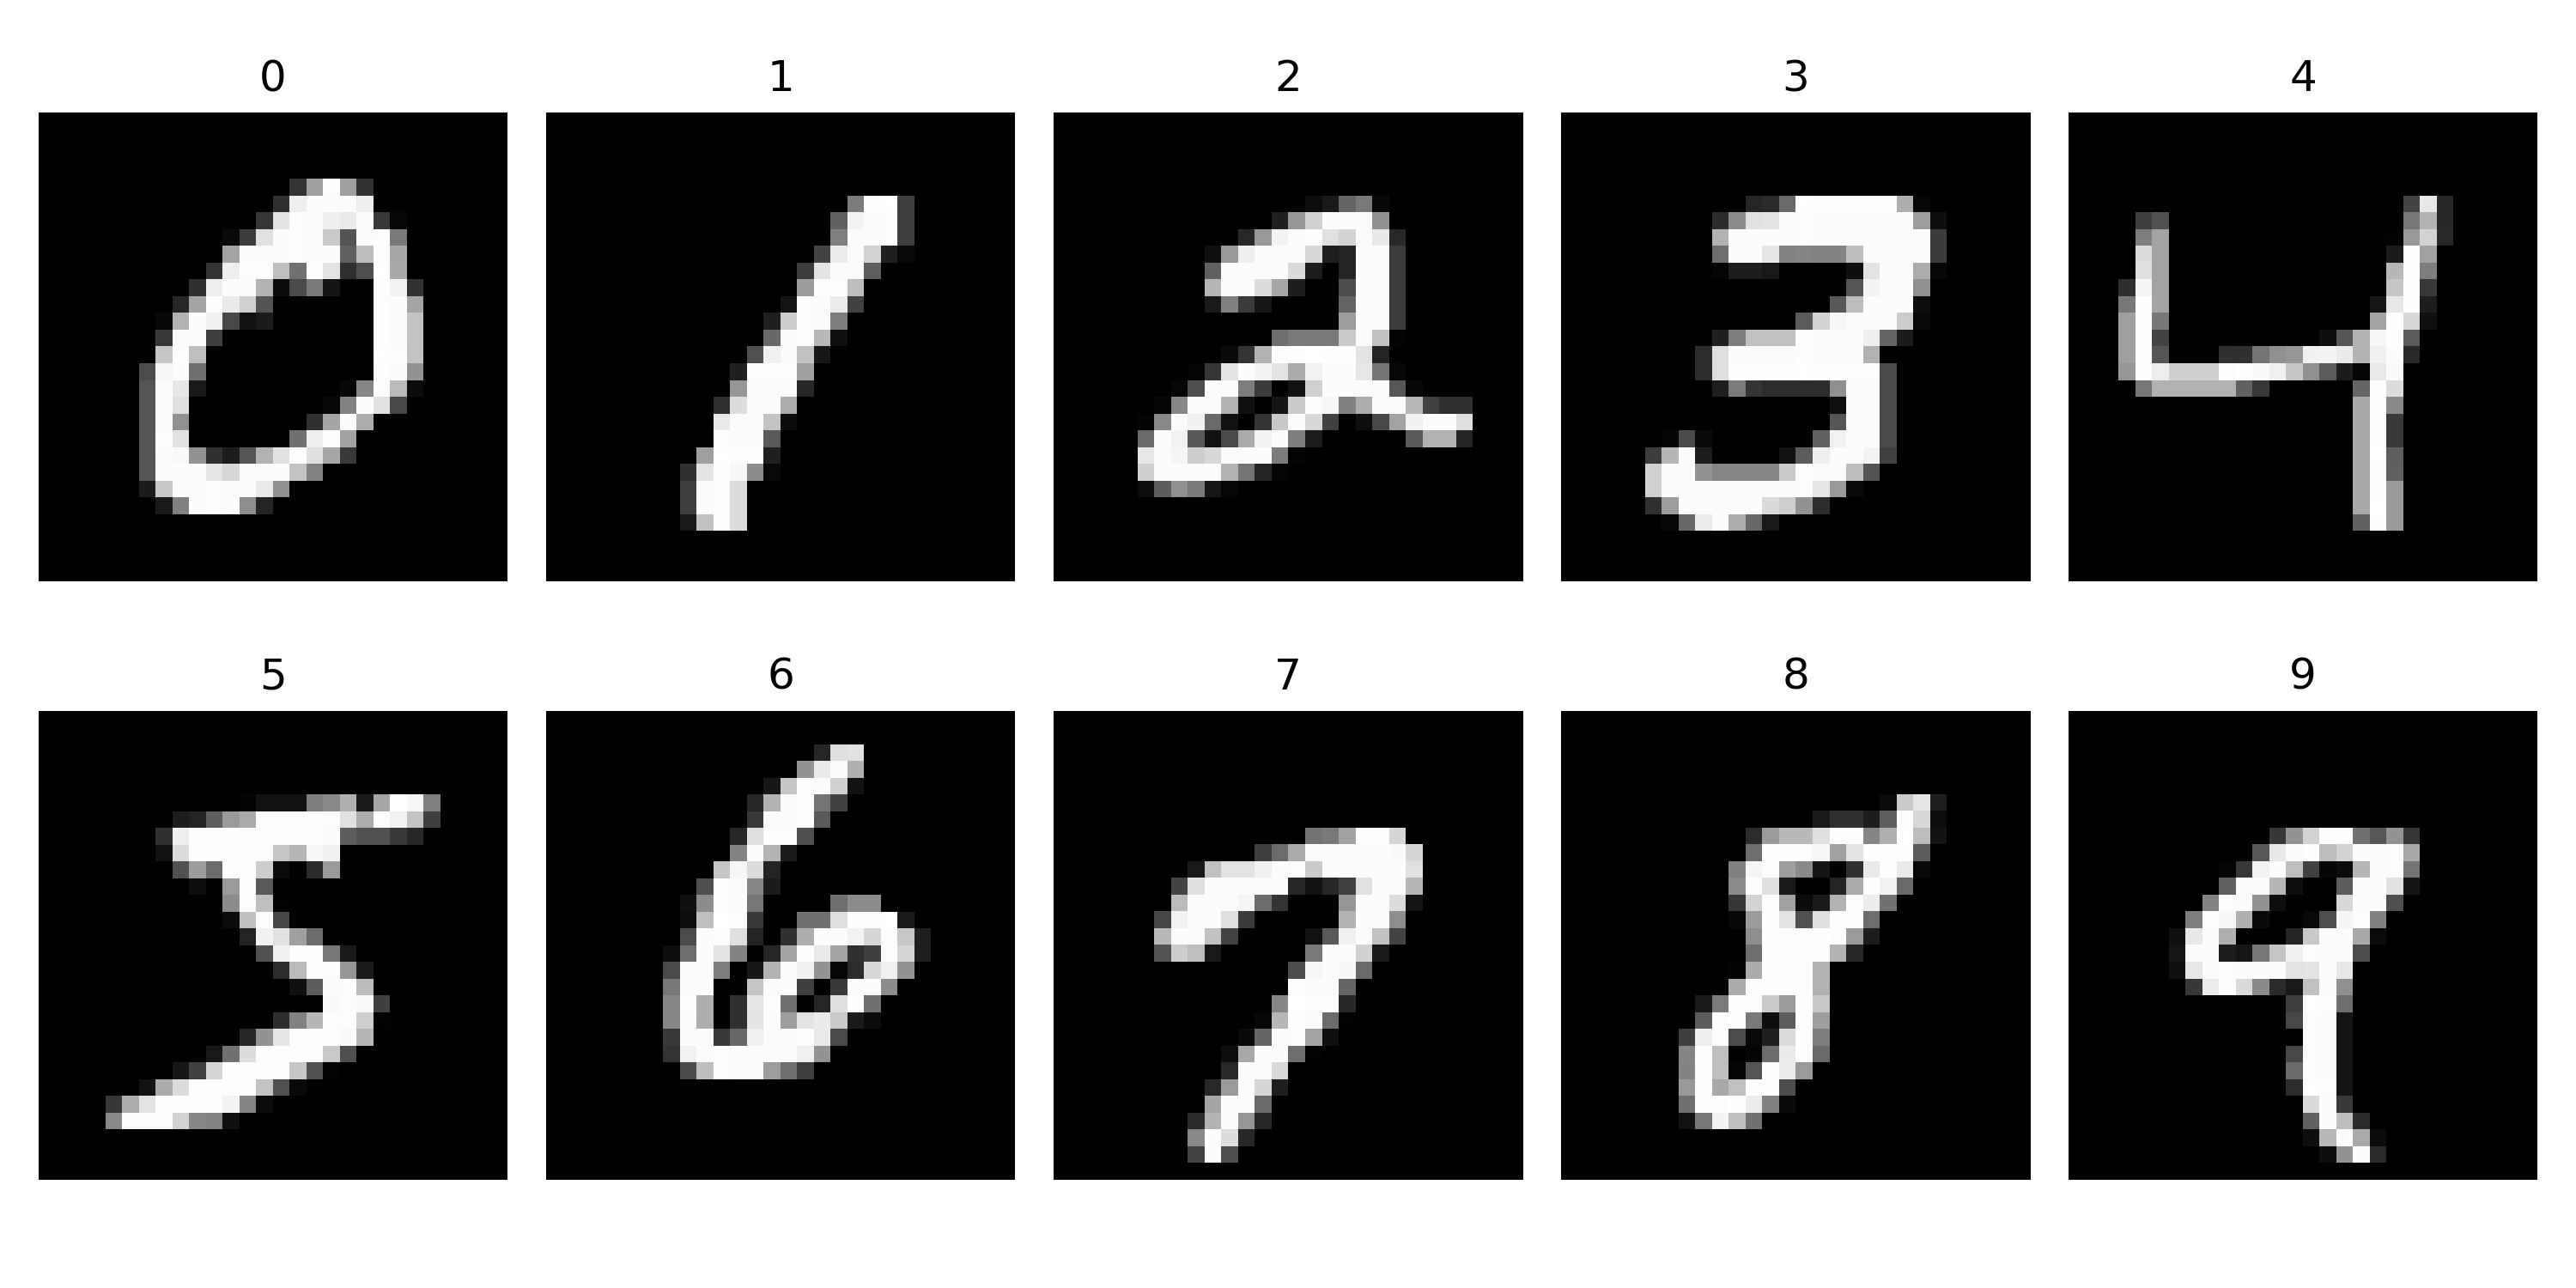
\includegraphics[width=0.48\textwidth]{MNIST_dataset.png}
	\caption{MNIST Dataset \cite{deng2012mnist}}
	\label{fig:mnist_dataset}
\end{figure}
The MNIST dataset is a widely used collection of handwritten digits that is commonly used for training and testing machine learning and computer vision algorithms. MNIST stands for the "Modified National Institute of Standards and Technology" database. It was created by modifying the original NIST dataset, which contained a much larger and more diverse set of handwritten characters, to focus specifically on handwritten digits.

The MNIST dataset contains 28x28-pixel grayscale images of handwritten digits (0 through 9), along with corresponding labels indicating which digit each image represents \cite{deng2012mnist}. There are 60,000 training images and 10,000 testing images in the MNIST dataset, making it a popular benchmark for various image classification tasks.
\subsubsection{ConvNet-3}
\subsubsection{Synthetic Dataset using real images}
\begin{figure}[H]
	\centering
	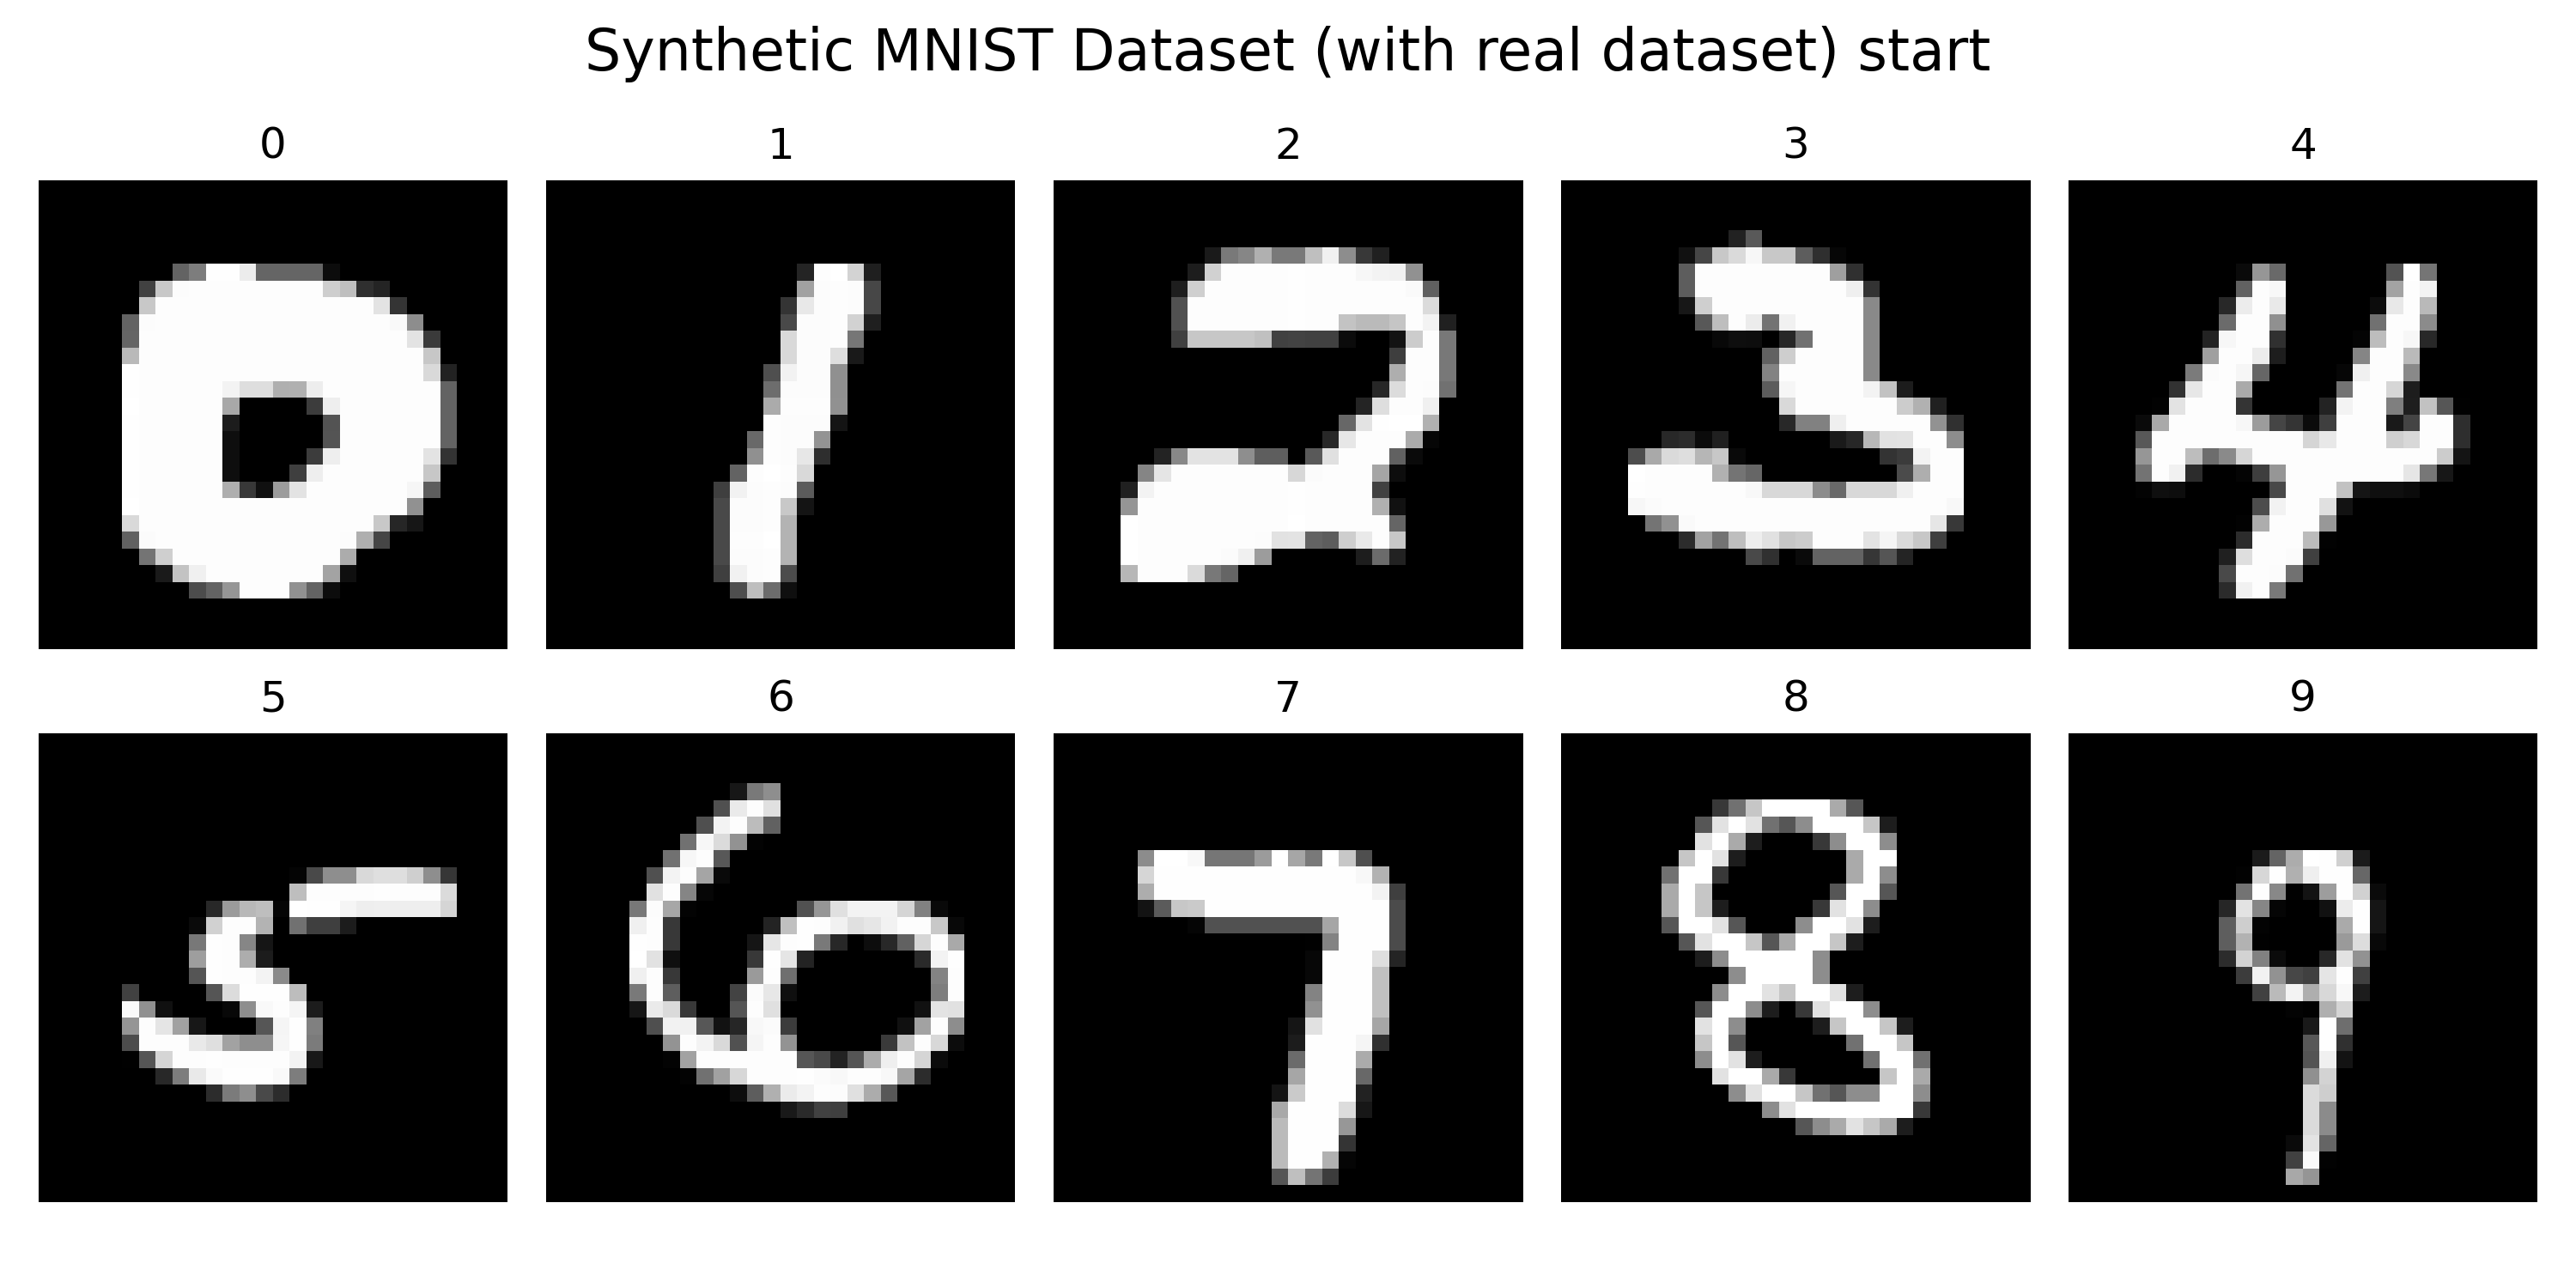
\includegraphics[width=0.48\textwidth]{mnist_real_sample.png}
	\caption{Sample of Synthetic MNIST Dataset created from real images (starting image)}
	\label{fig:mnist_real_sample}
\end{figure}

\begin{figure}[H]
	\centering
	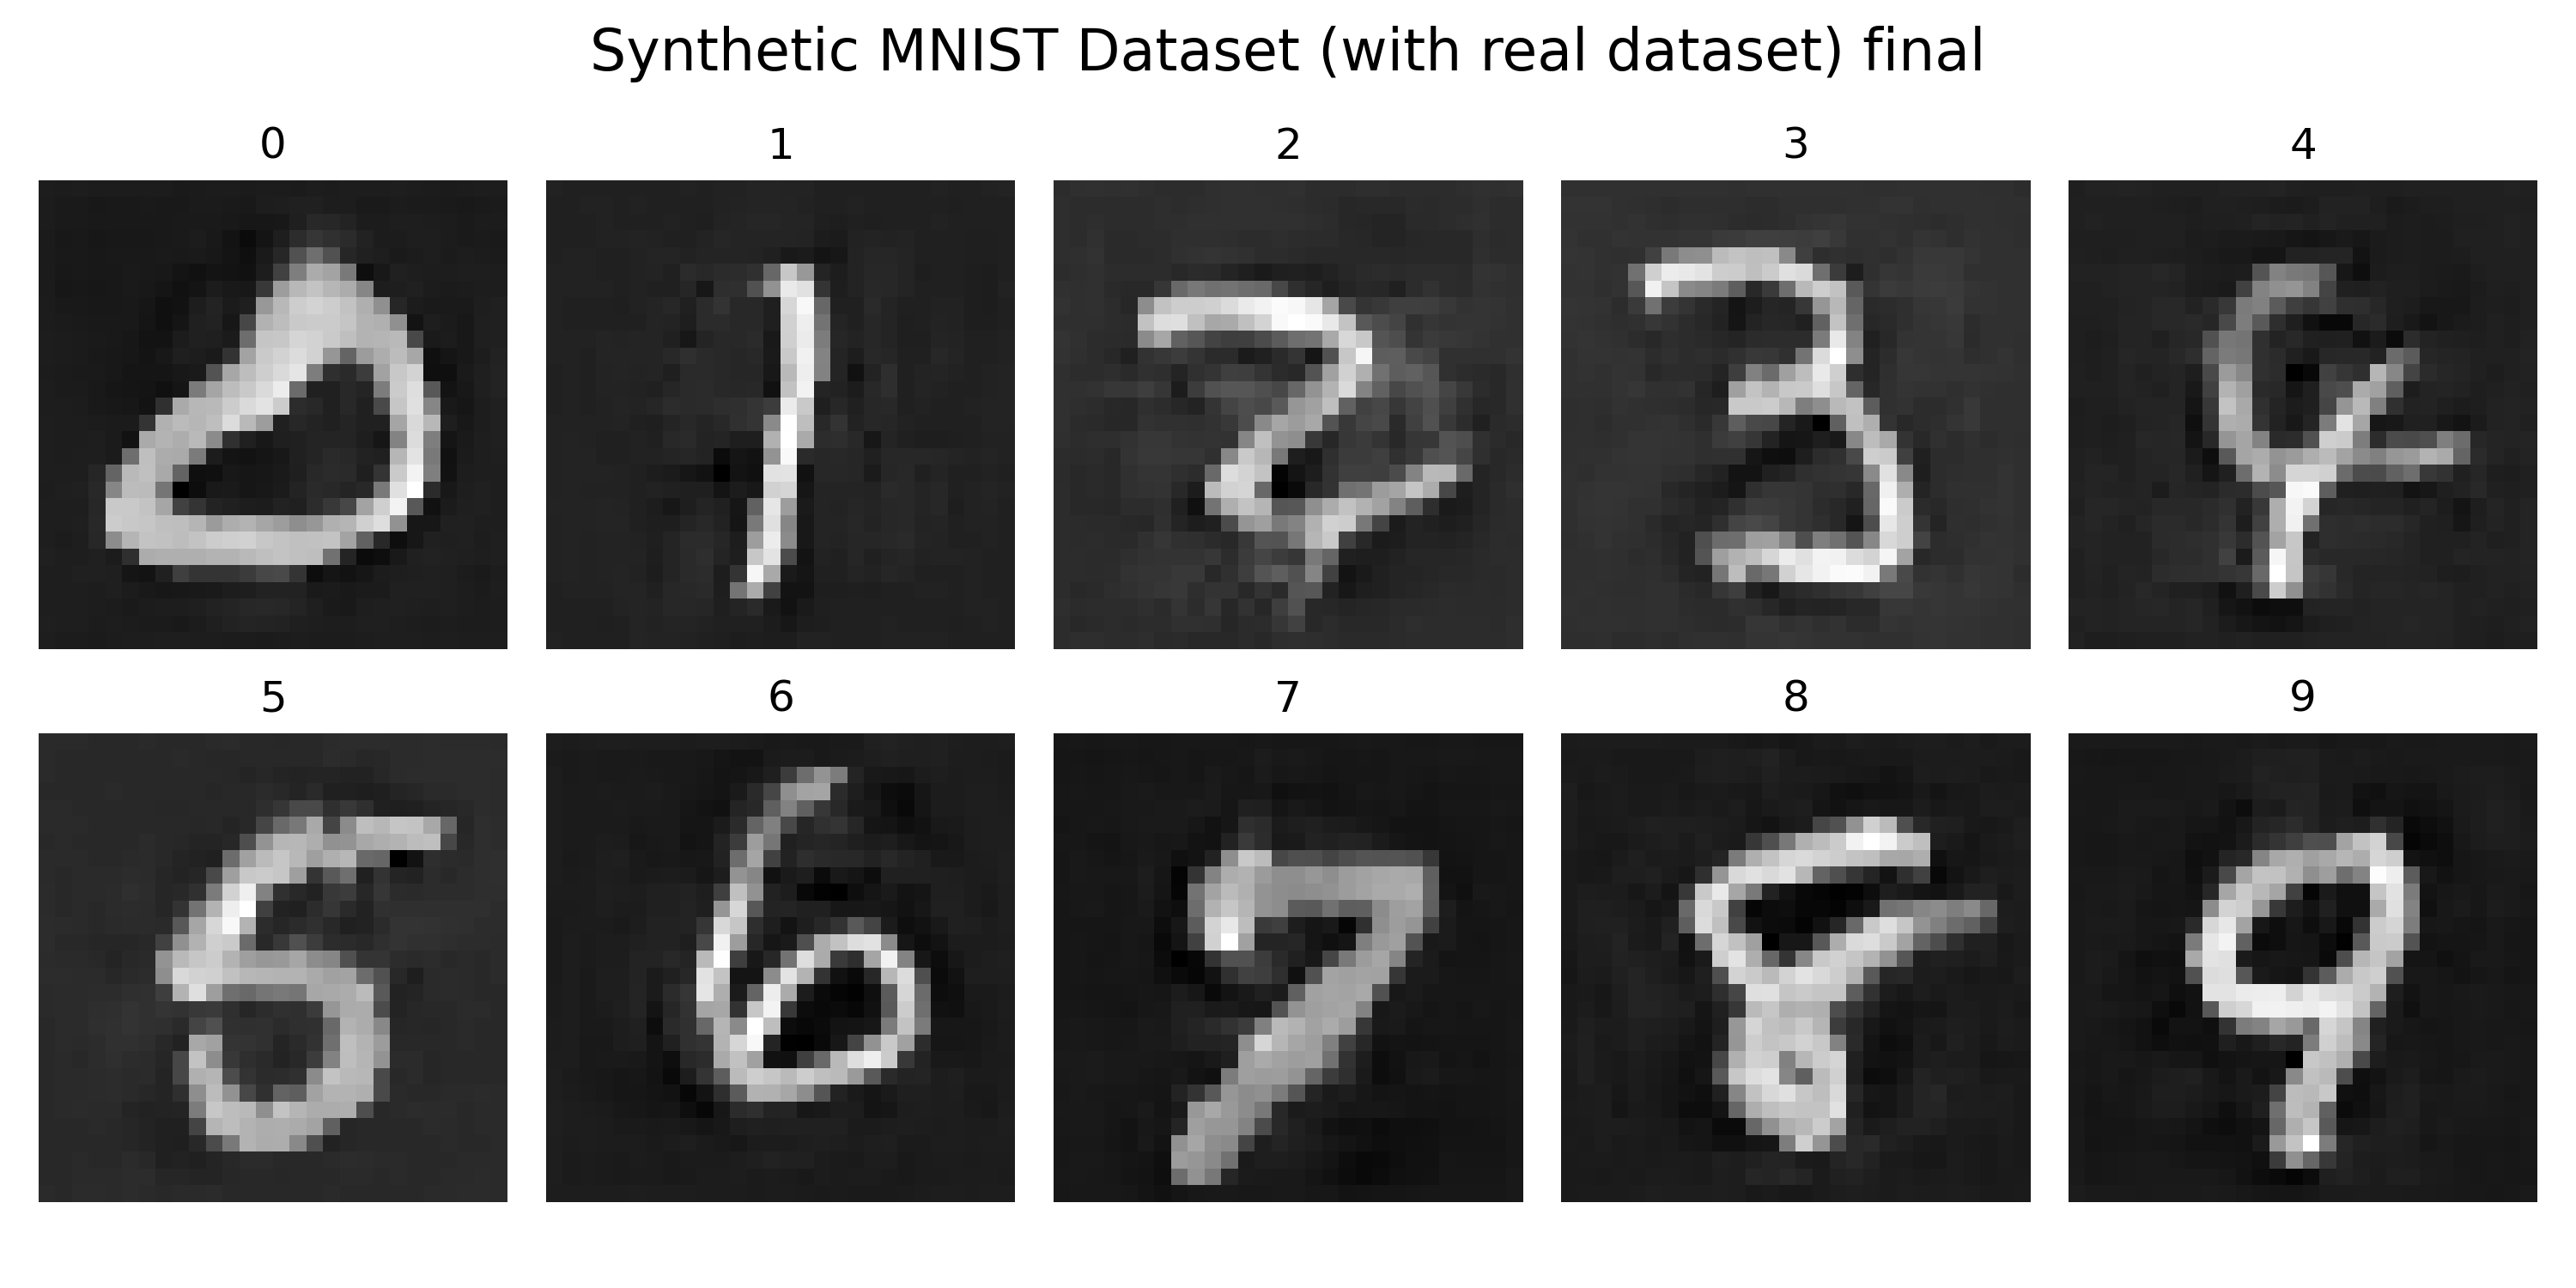
\includegraphics[width=0.48\textwidth]{mnist_real_syn.png}
	\caption{Sample of Synthetic MNIST Dataset created from real images (final image)}
	\label{fig:mnist_real_syn}
\end{figure}

\begin{figure}[H]
	\centering
	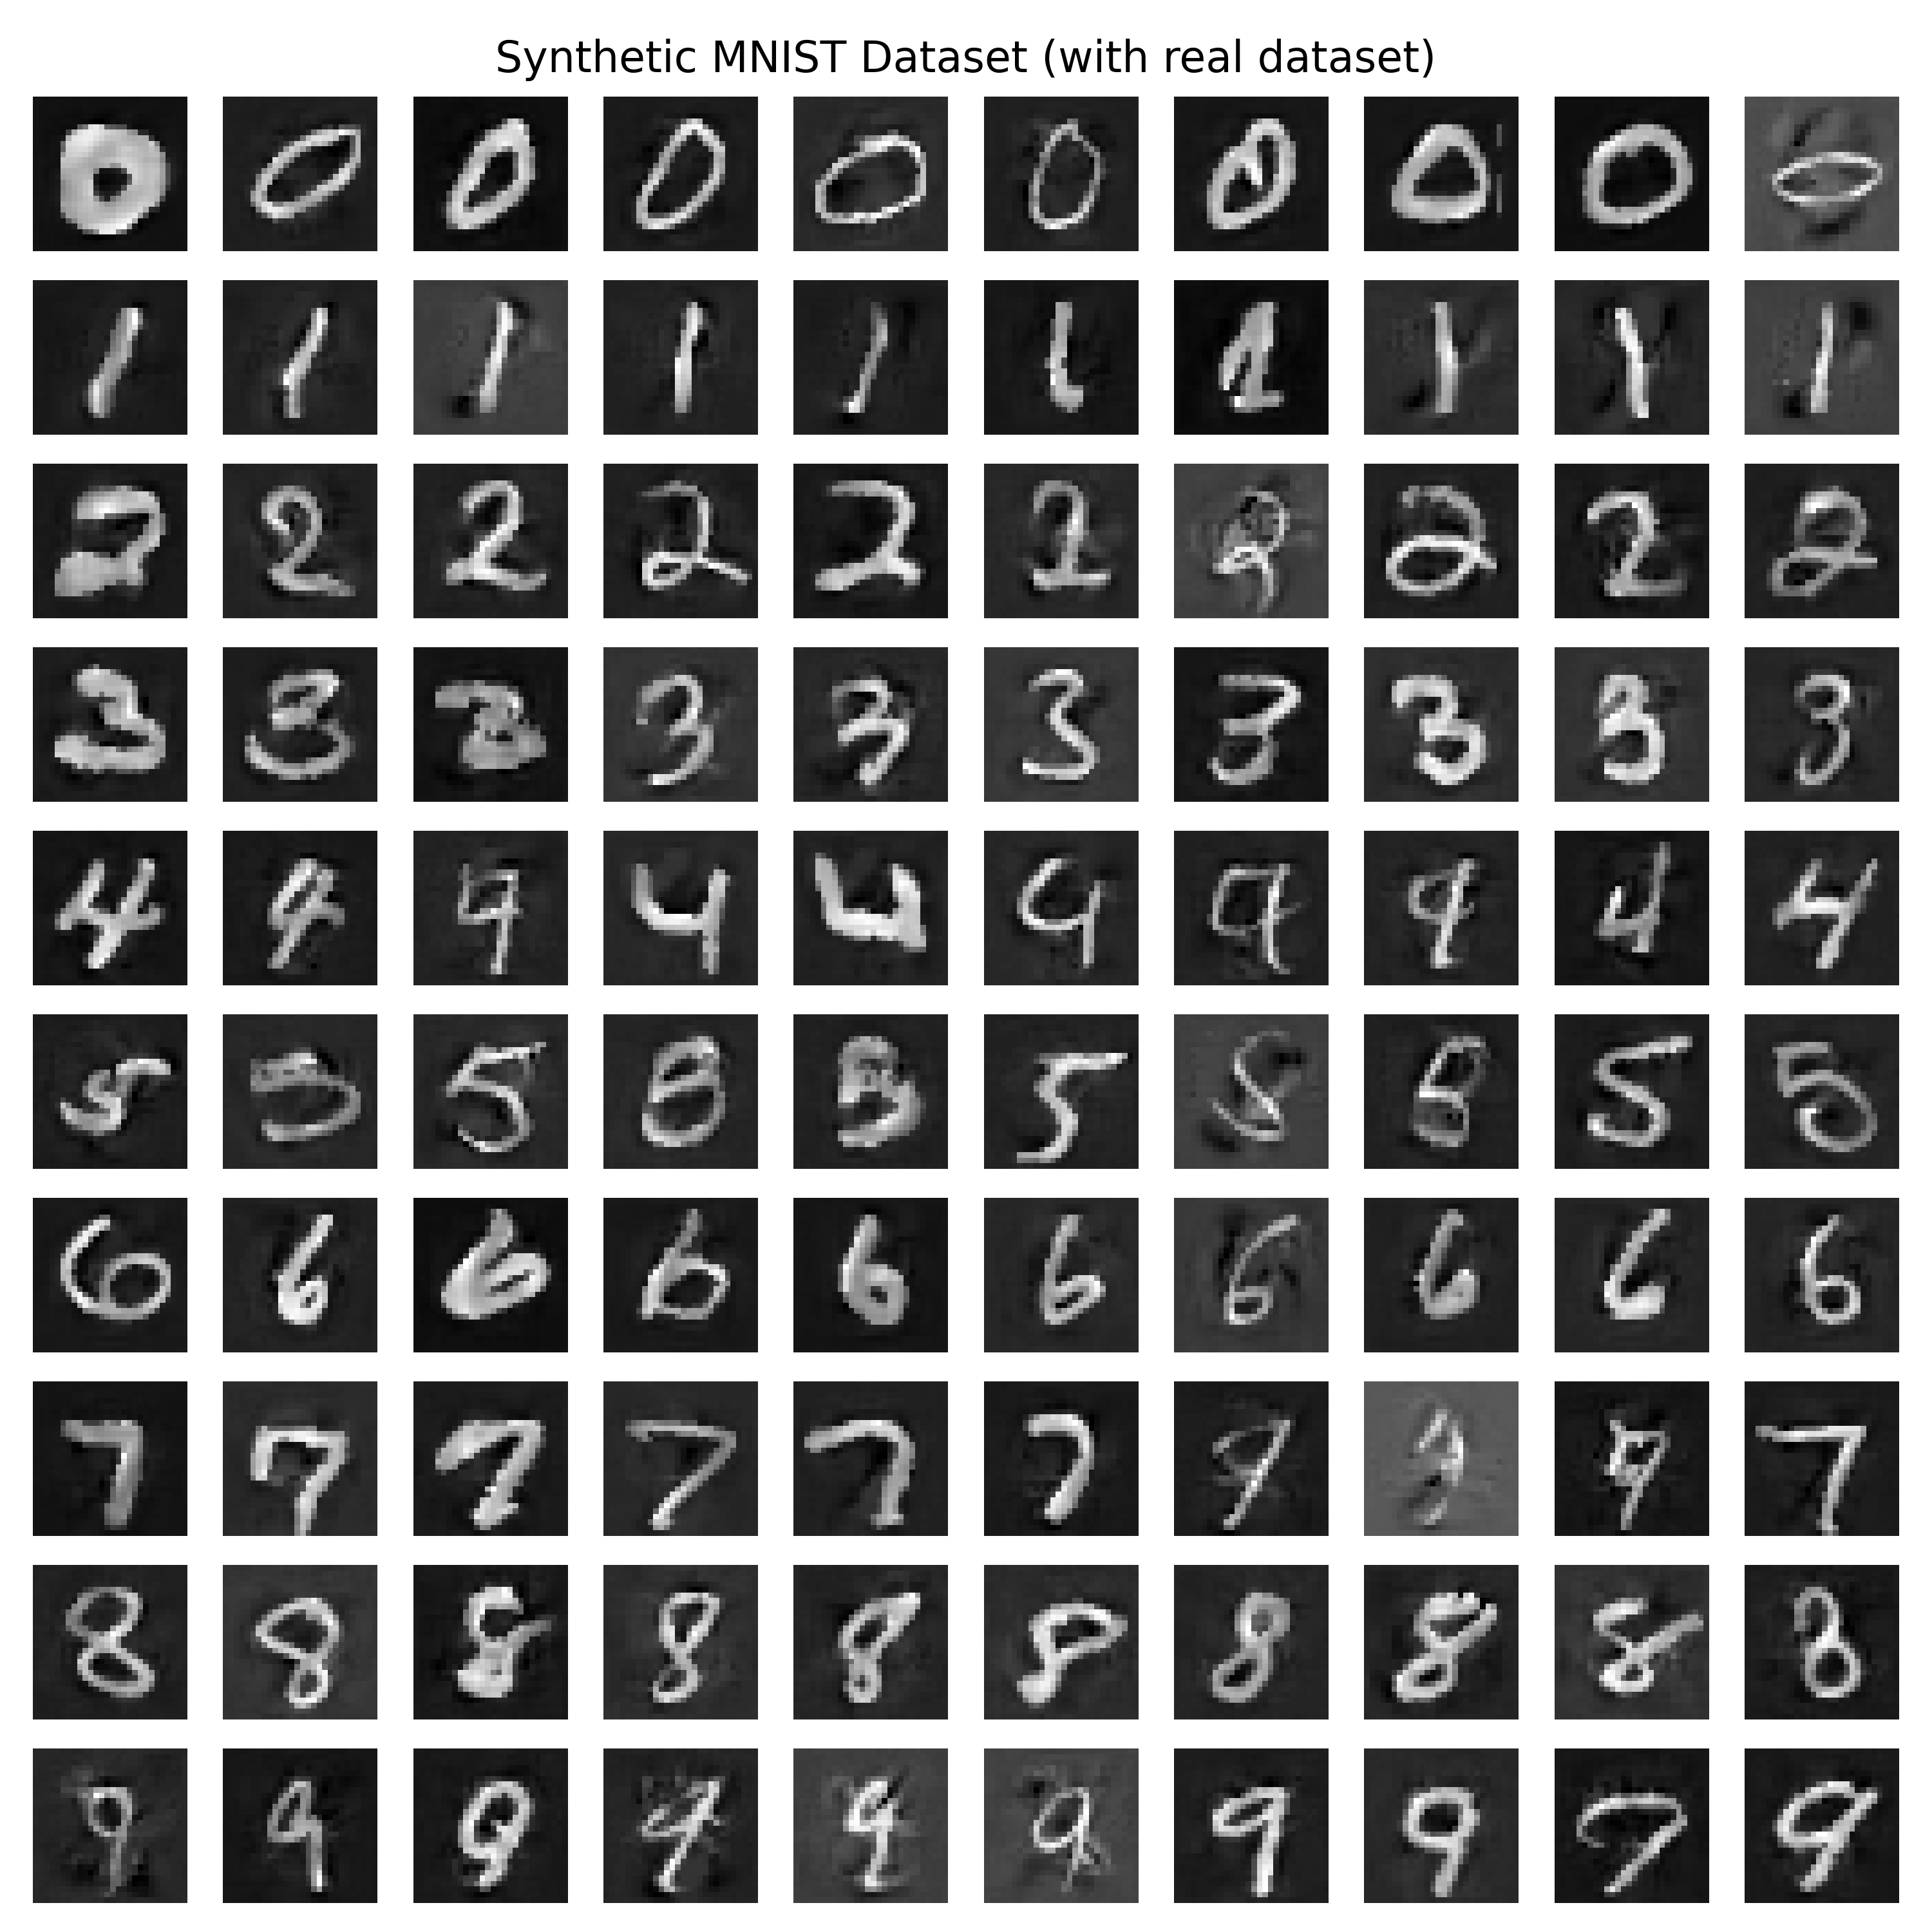
\includegraphics[width=0.48\textwidth]{mnist_real_syn_all.png}
	\caption{Synthetic MNIST Dataset created from real images}
	\label{fig:mnist_real_syn_all}
\end{figure}
\subsubsection{Synthetic Dataset using Gaussian noise}
\begin{figure}[H]
	\centering
	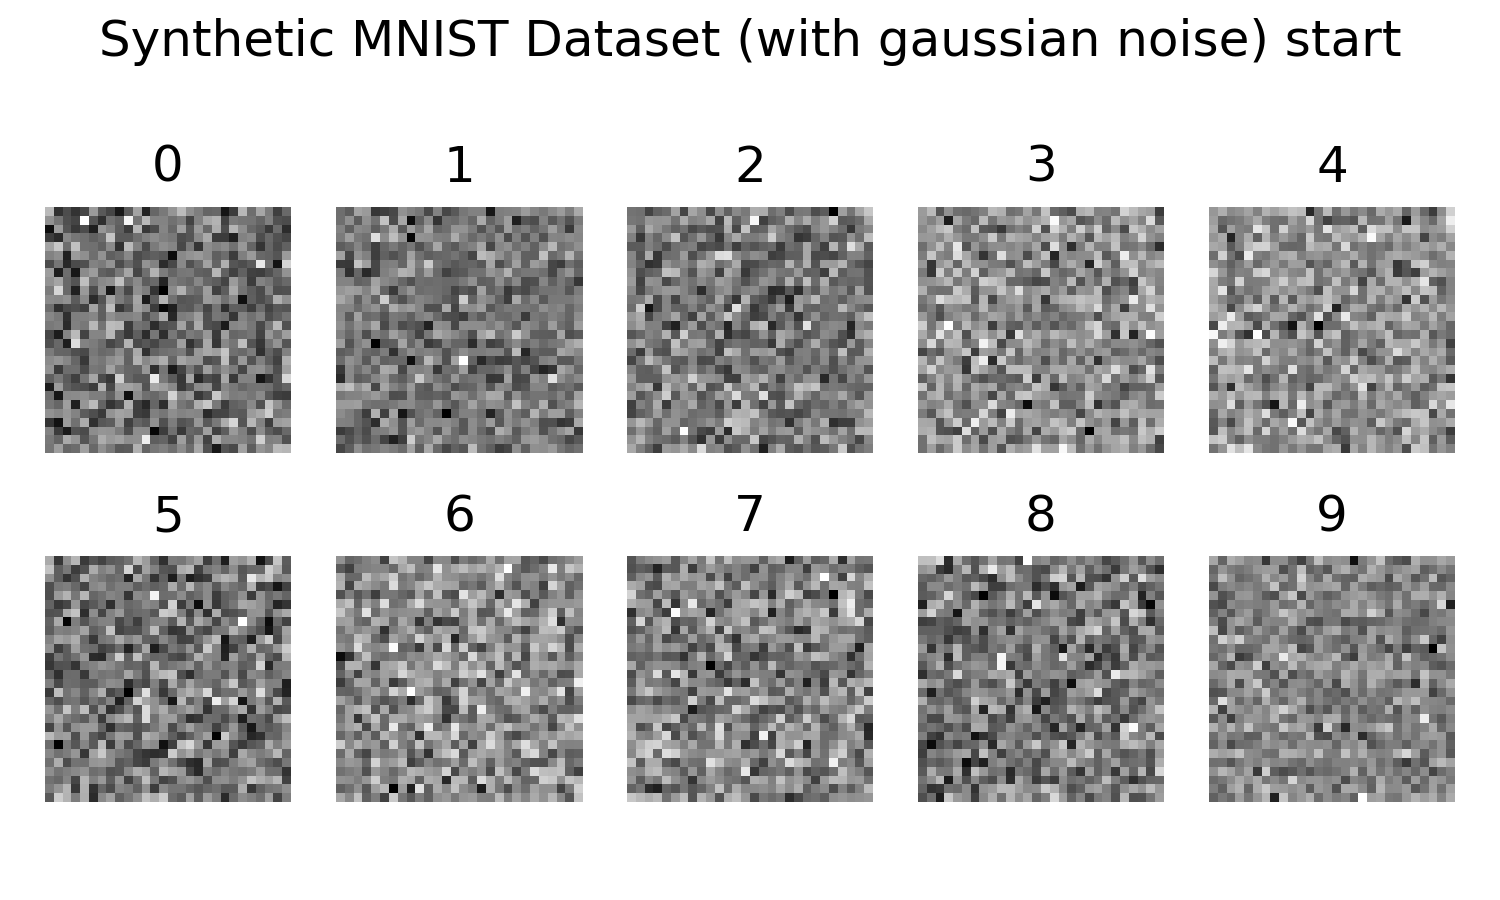
\includegraphics[width=0.48\textwidth]{mnist_noise_sample.png}
	\caption{Sample of Synthetic MNIST Dataset created from Gaussian noise (starting image)}
	\label{fig:mnist_noise_sample}
\end{figure}

\begin{figure}[H]
	\centering
	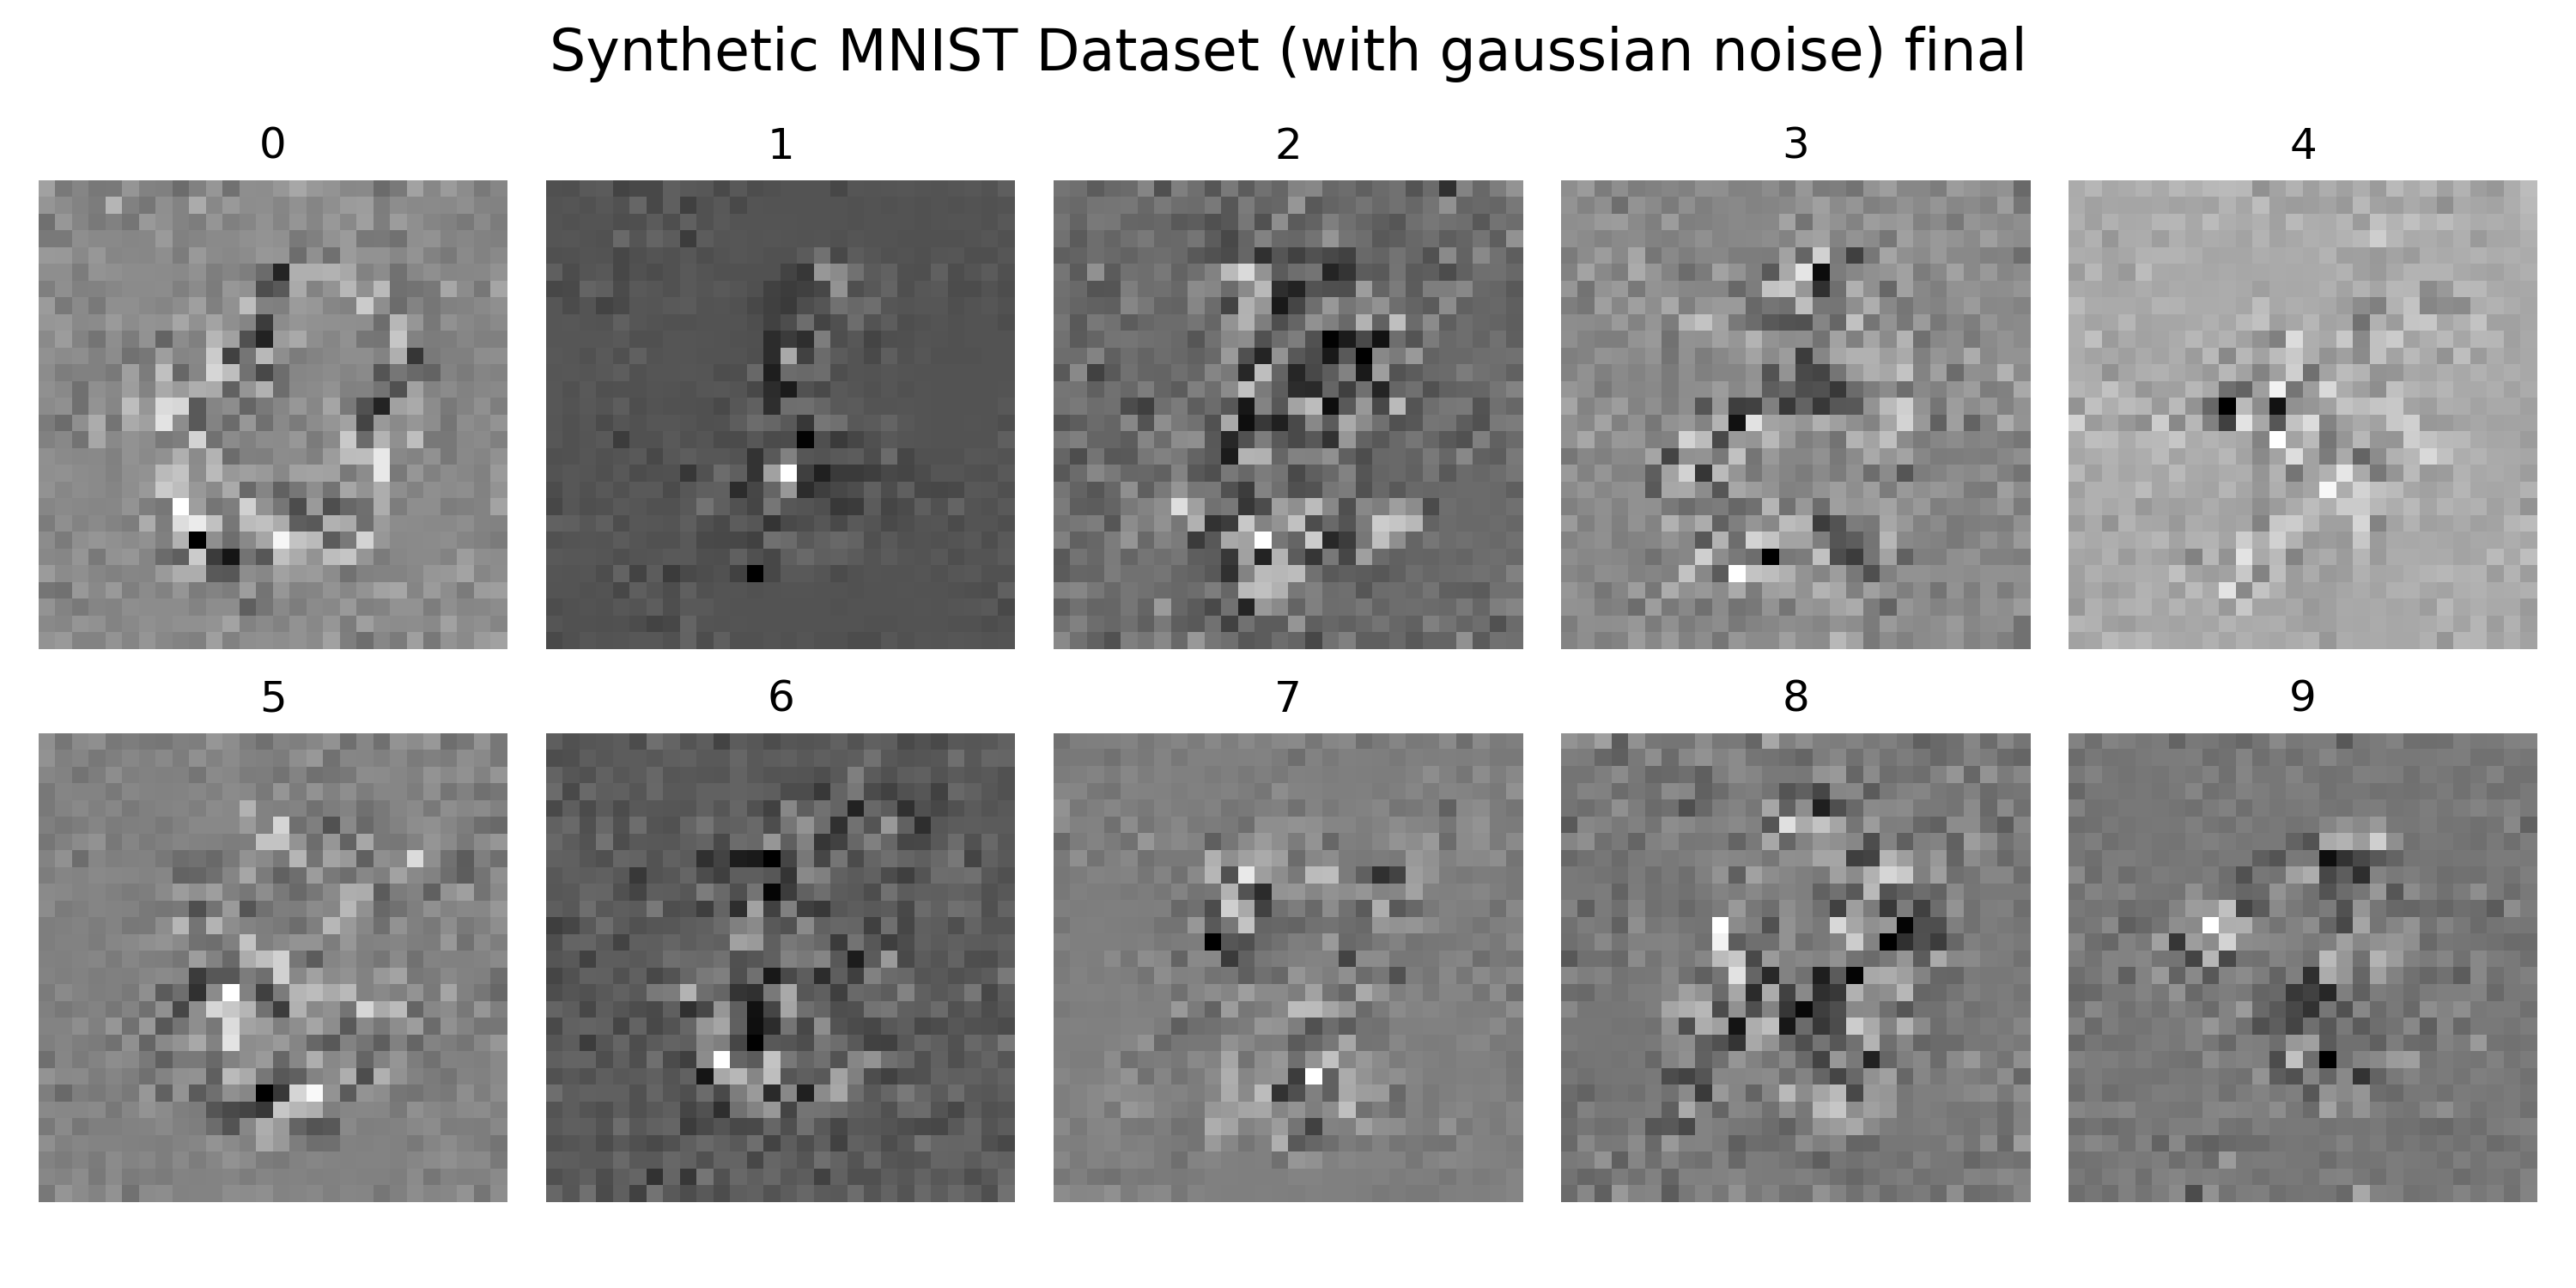
\includegraphics[width=0.48\textwidth]{mnist_noise_syn.png}
	\caption{Sample of Synthetic MNIST Dataset created from Gaussian noise (final image)}
	\label{fig:mnist_noise_syn}
\end{figure}

\begin{figure}[H]
	\centering
	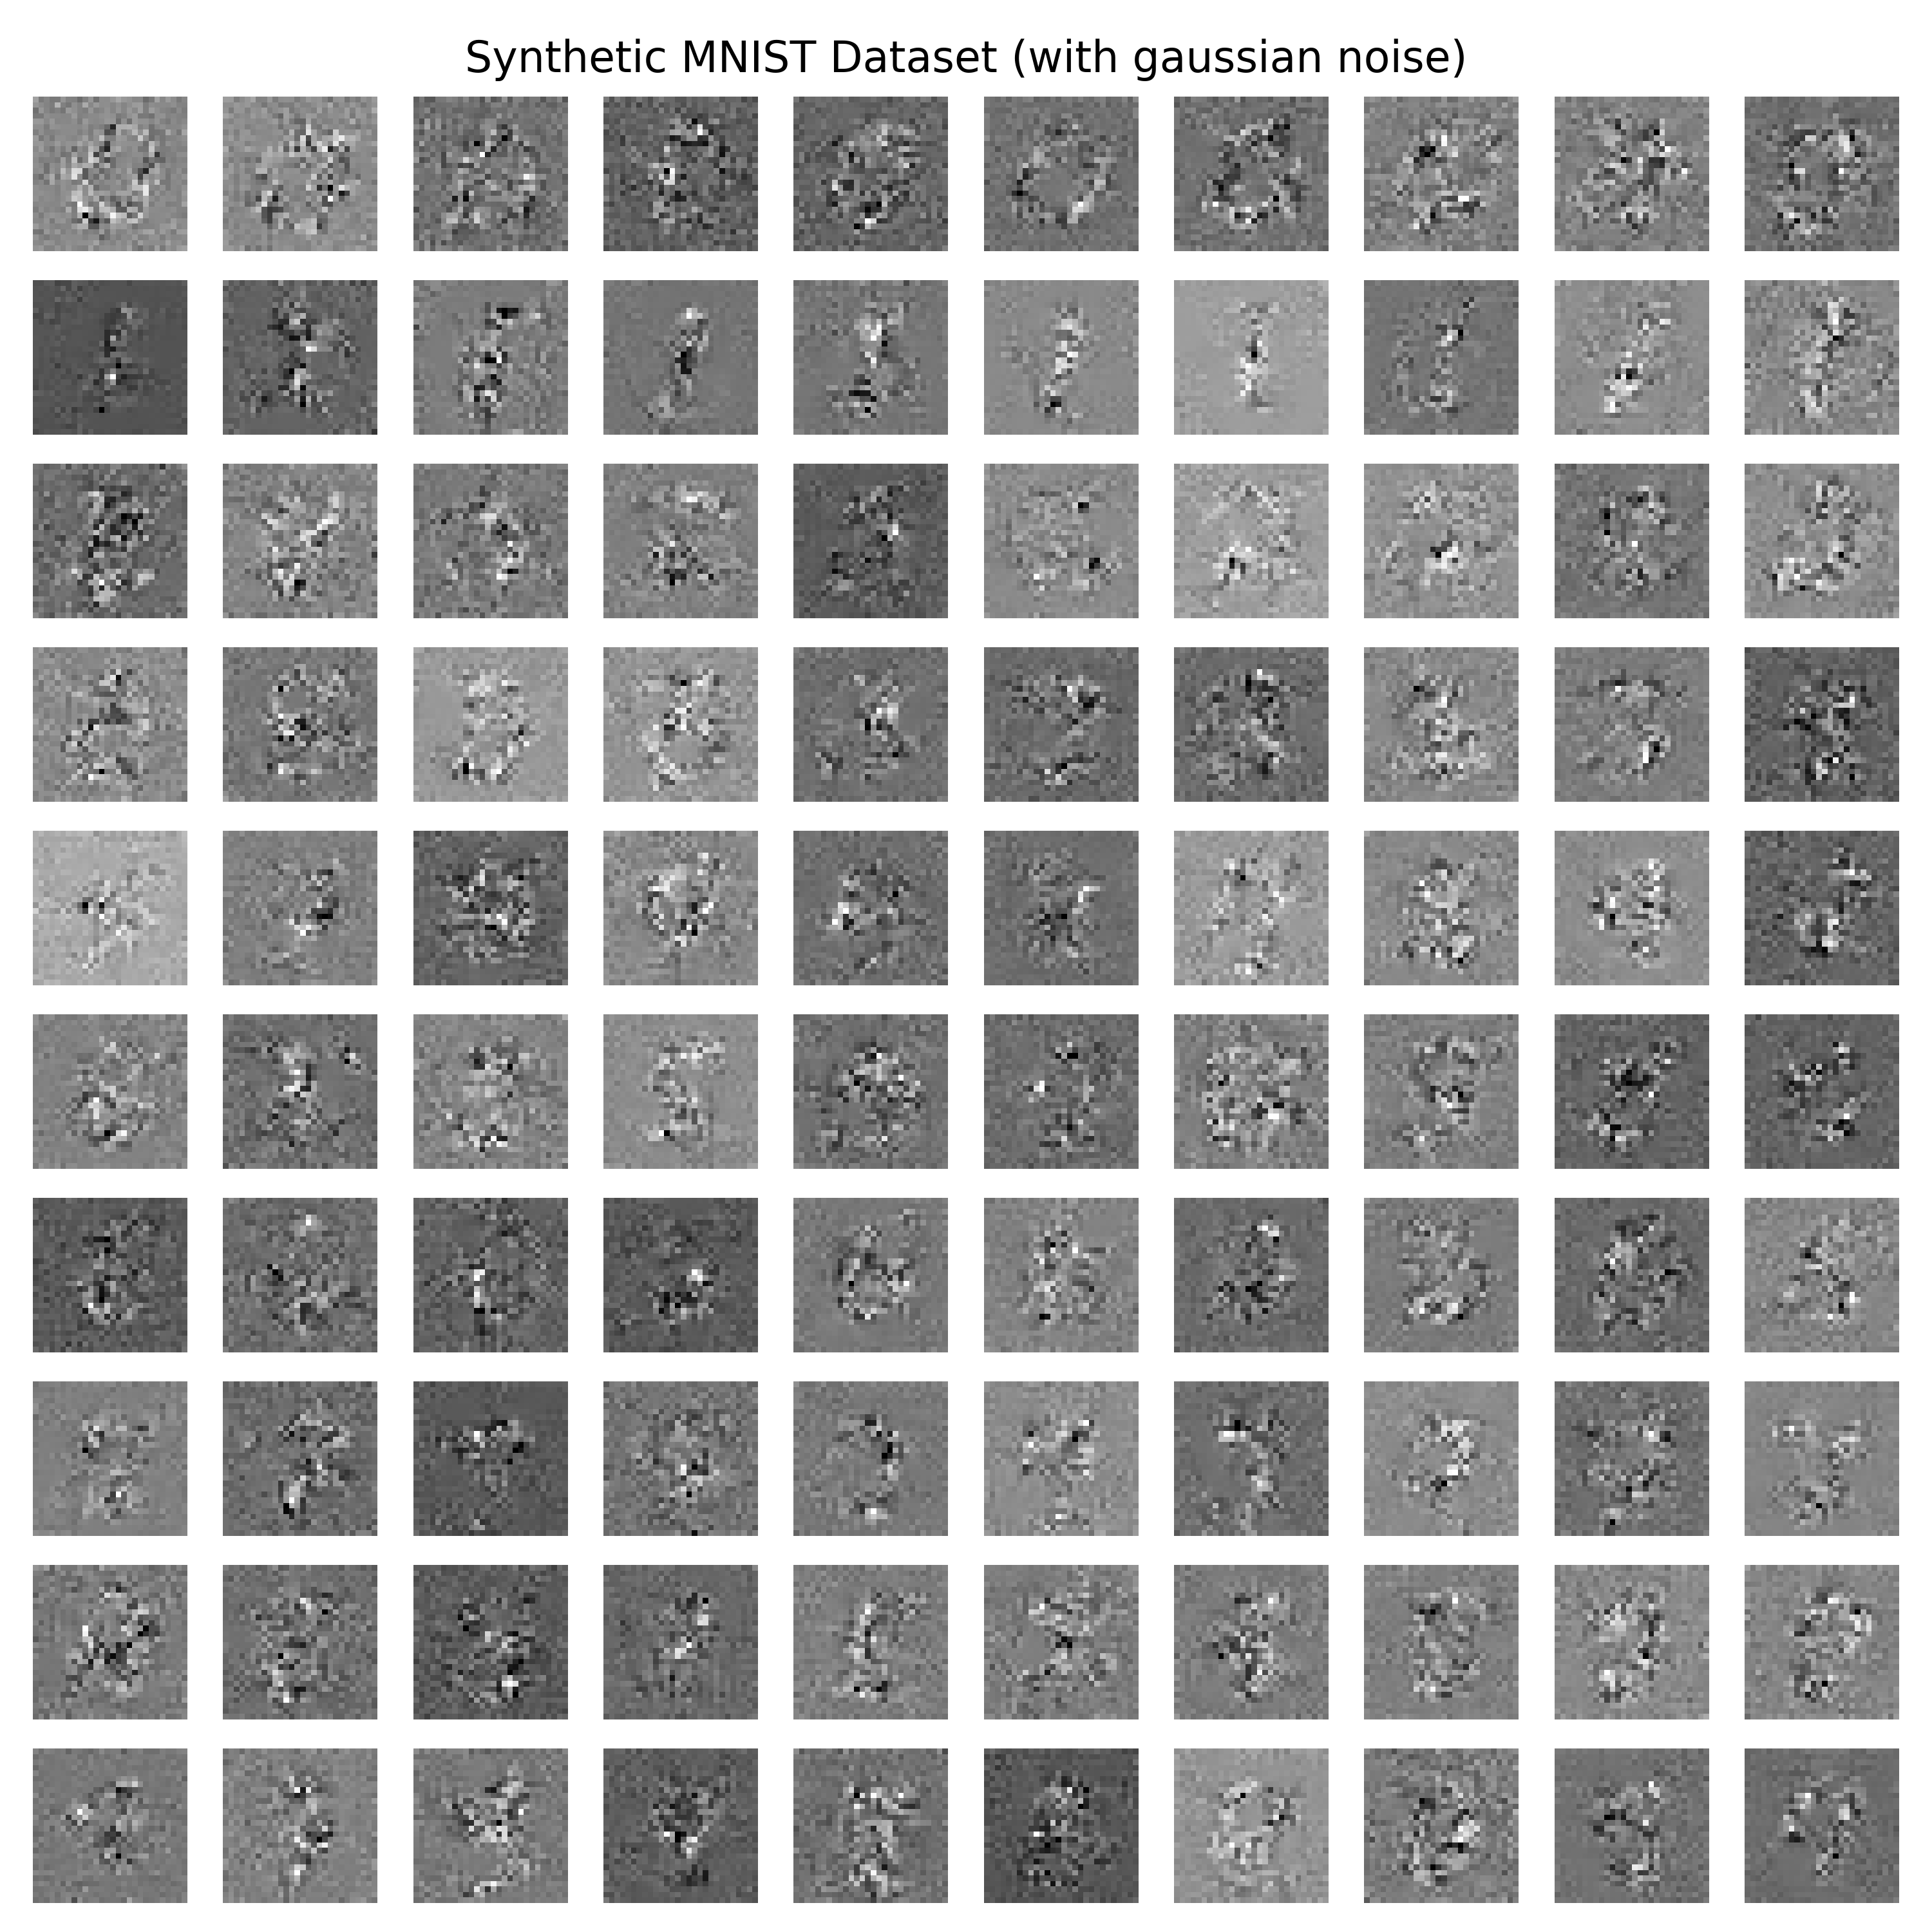
\includegraphics[width=0.48\textwidth]{mnist_noise_syn_all.png}
	\caption{Synthetic MNIST Dataset created from Gaussian noise}
	\label{fig:mnist_noise_syn_all}
\end{figure}
\subsubsection{ConvNet-3 using Synthetic Dataset}
\begin{figure}[H]
	\centering
	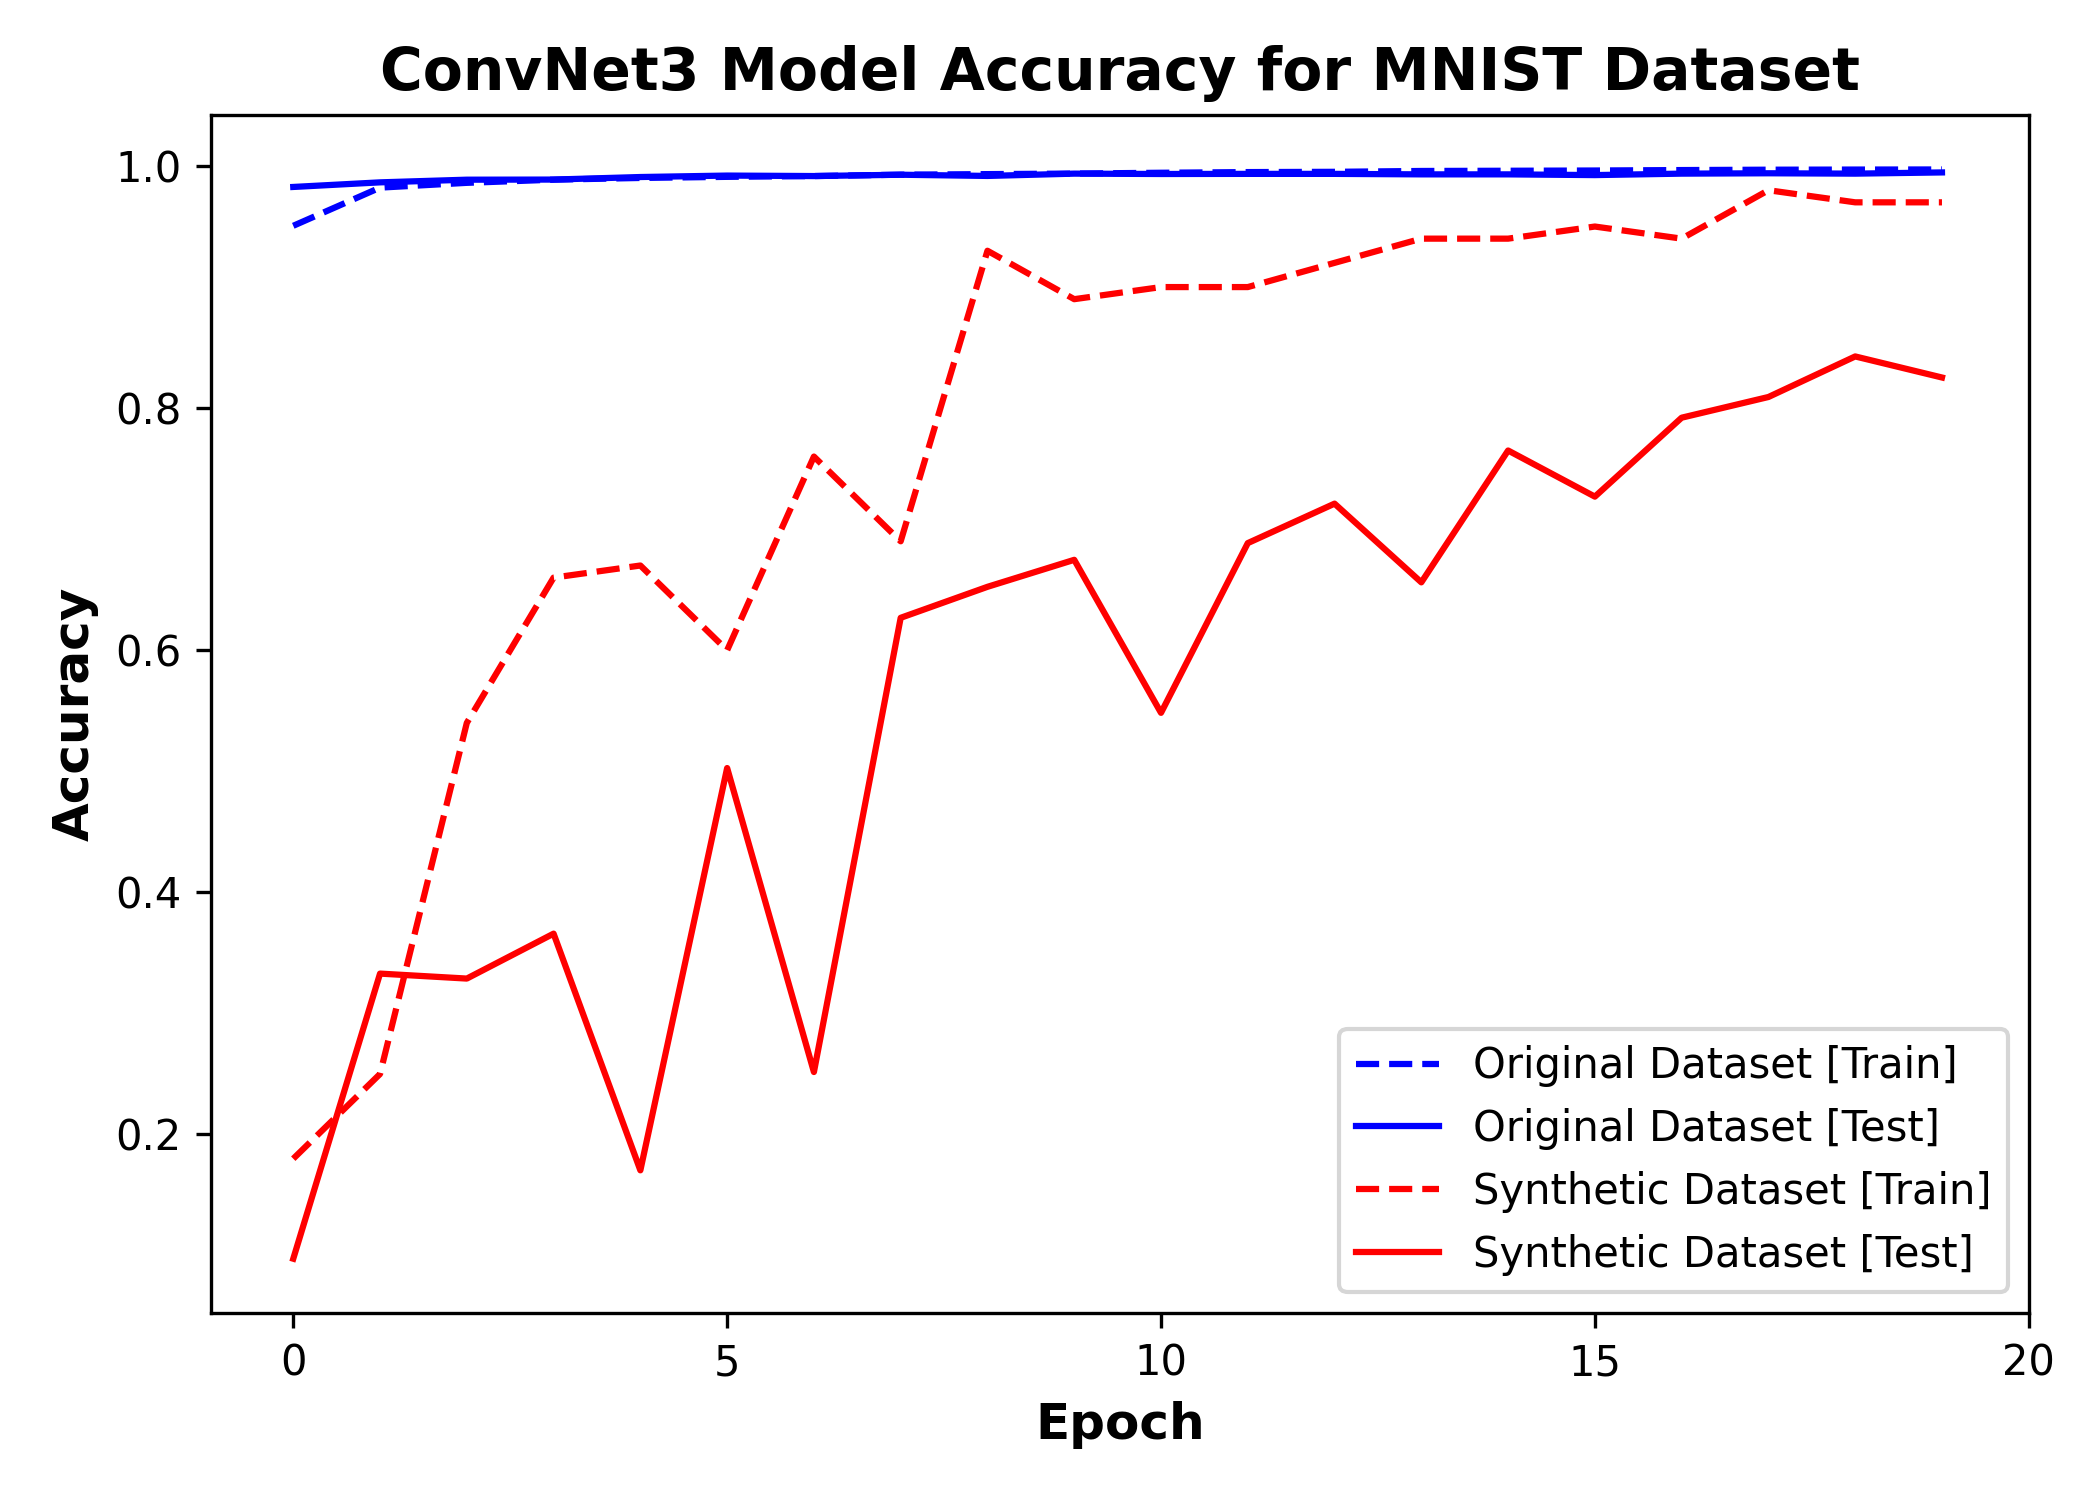
\includegraphics[width=0.48\textwidth]{mnist_syn_acc.png}
	\caption{ConvNet-3 Model Trained using Original and Synthetic dataset}
	\label{fig:mnist_syn_acc}
\end{figure}
\subsubsection{Cross-architecture Generalization - AlexNet}
\begin{figure}[H]
	\centering
	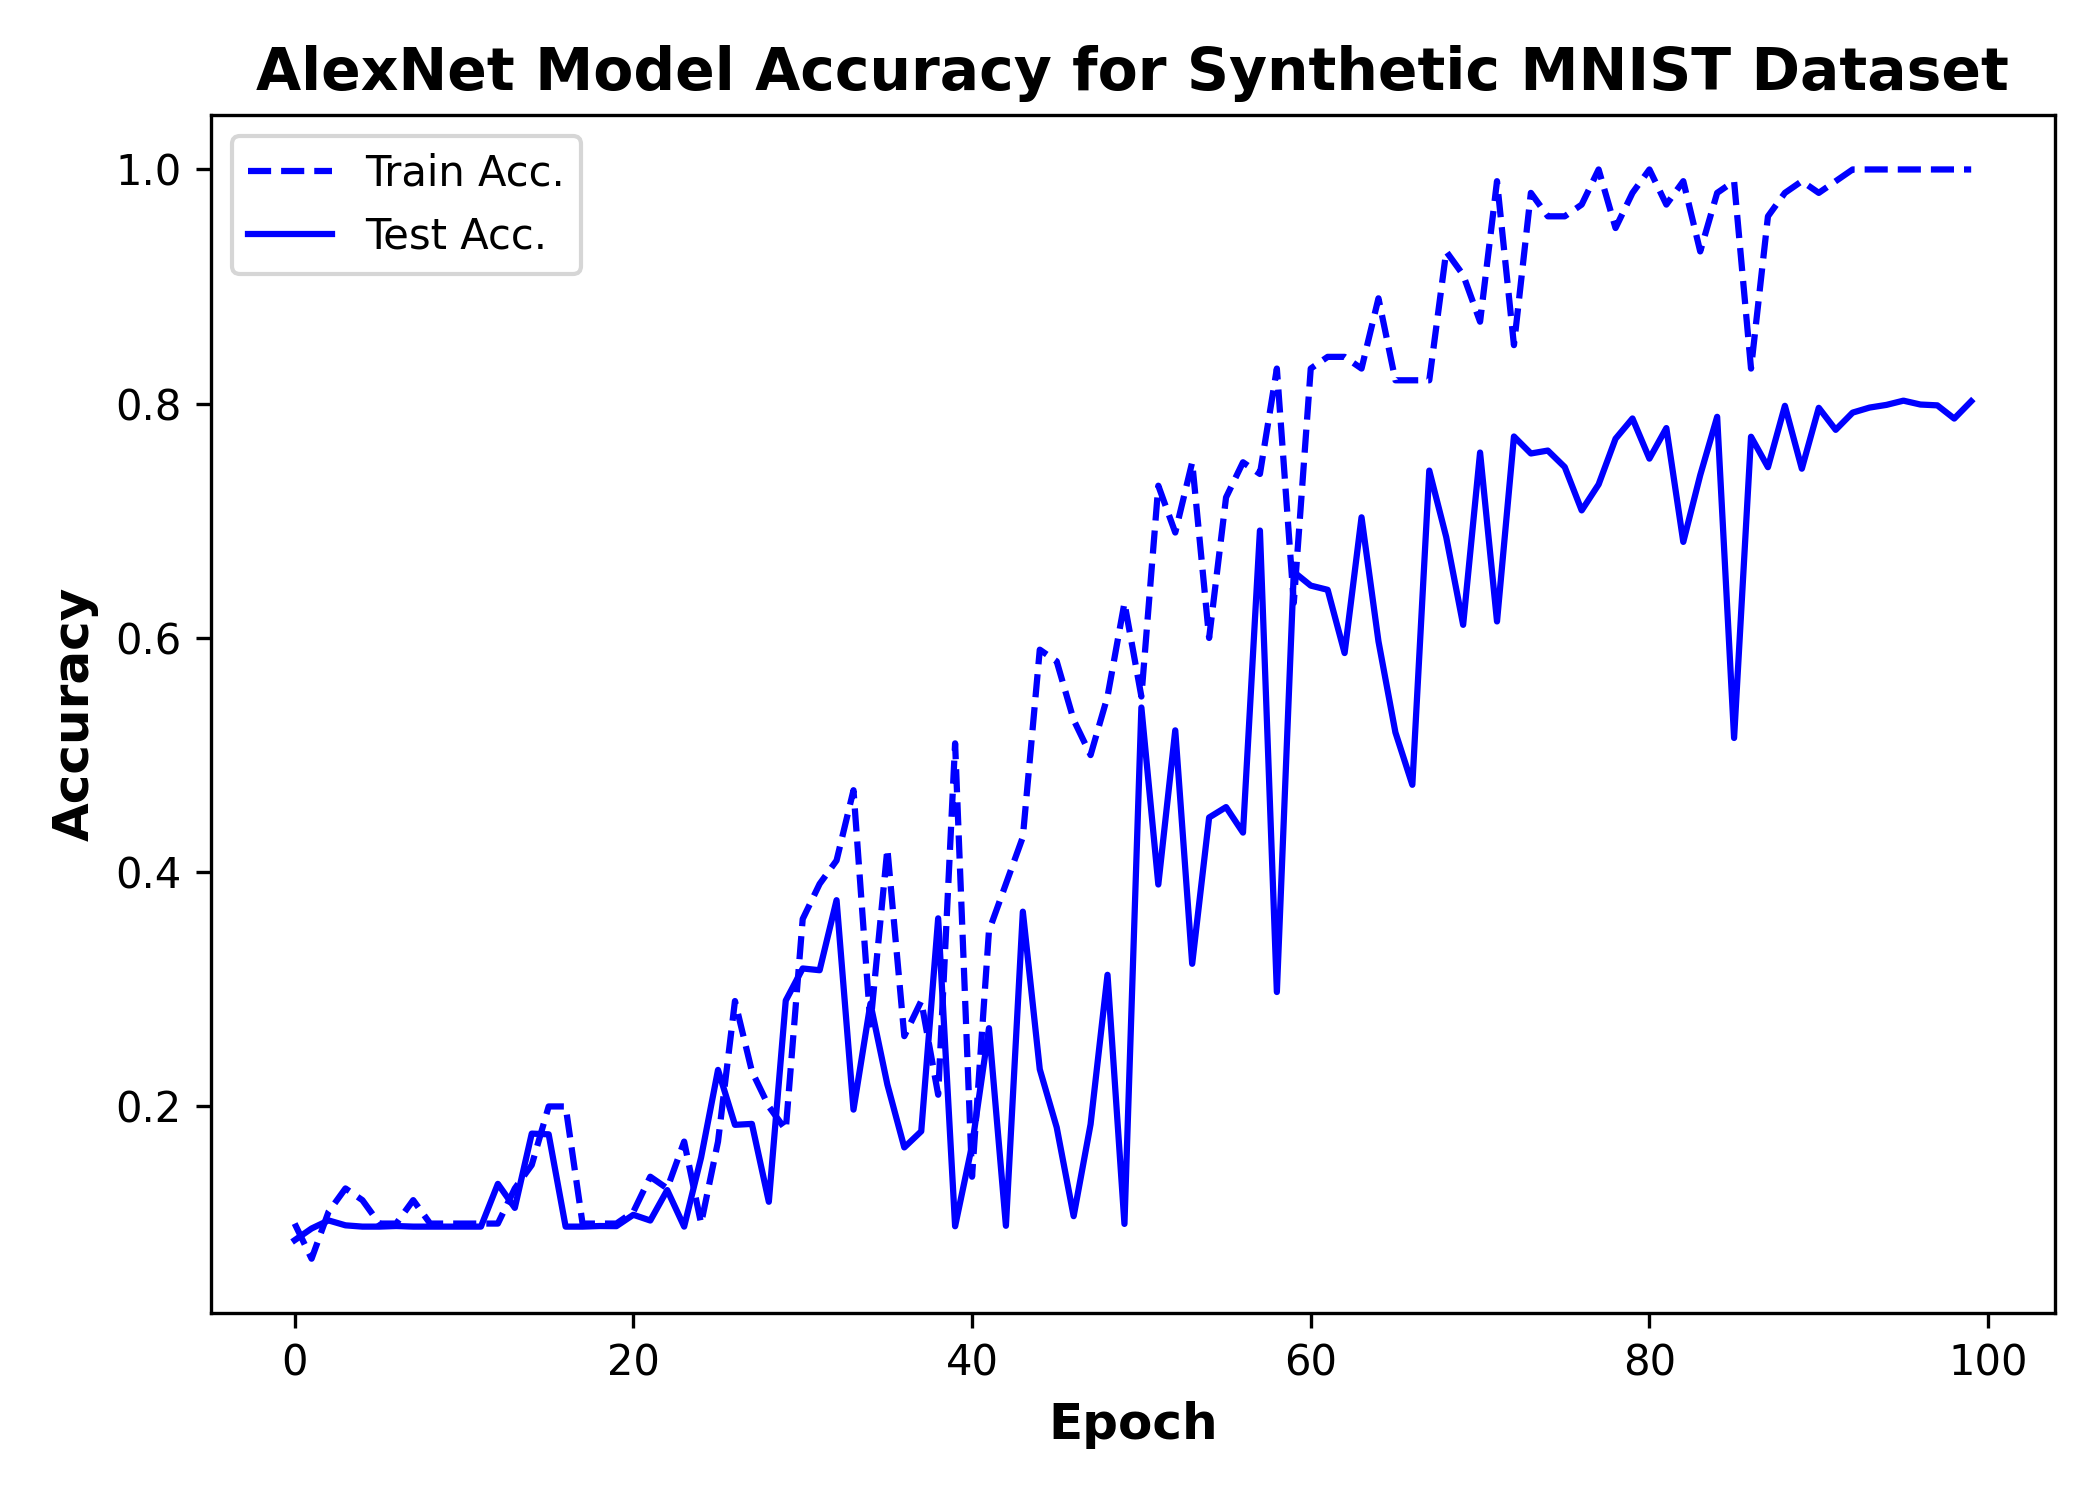
\includegraphics[width=0.48\textwidth]{mnist_alex_acc.png}
	\caption{AlexNet Model Trained using Synthetic dataset}
	\label{fig:mnist_alex_acc}
\end{figure}
\subsection{MHIST Dataset}
The MHIST dataset, short for "Minimalist Histopathology Image Screening Test," is a specialized dataset commonly used for training and evaluating machine learning models in the field of digital pathology. It was developed to address specific challenges in histopathological image analysis, focusing particularly on the differentiation between types of colorectal polyp tissues.

The MHIST dataset contains 224x224-pixel RGB images of hematoxylin and eosin (H\&E) stained histopathology slides, with labels distinguishing between two classes: hyperplastic (non-cancerous) and adenomatous (pre-cancerous) polyps. It consists of 3,152 image patches divided into 2,456 training images and 696 testing images, making it a valuable resource for binary classification tasks in medical image analysis \cite{wei2021petri}.
\begin{figure}[H]
	\centering
	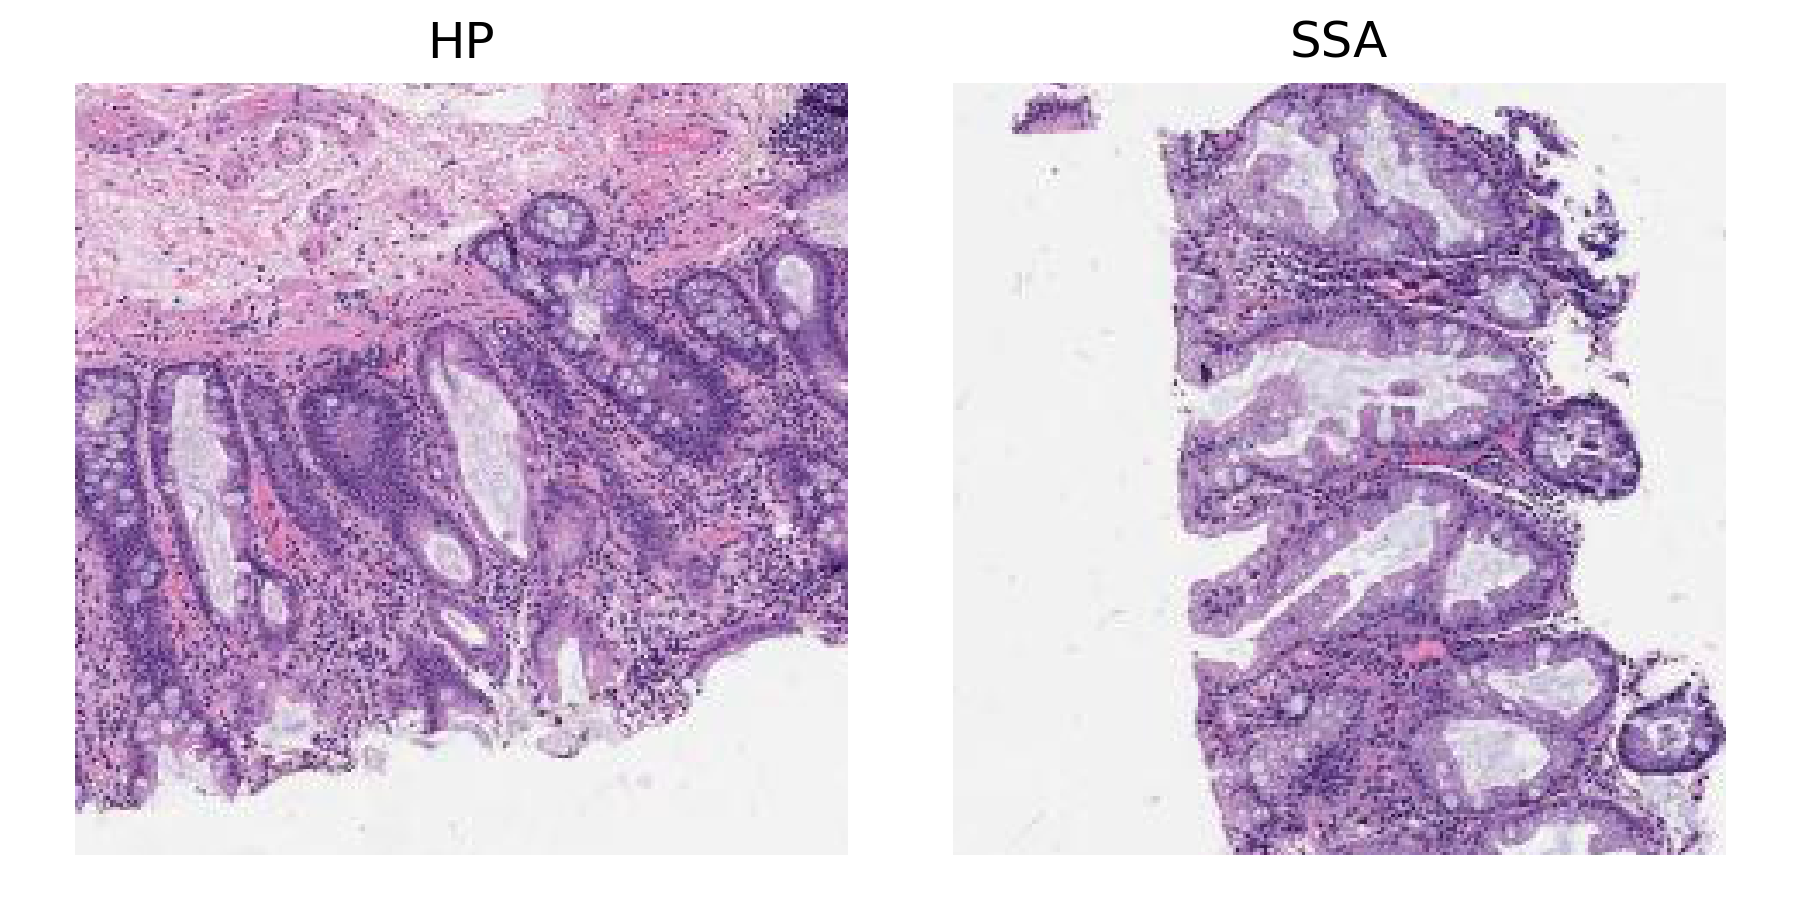
\includegraphics[width=0.48\textwidth]{MHIST_dataset.png}
	\caption{MHIST Dataset \cite{wei2021petri}}
	\label{fig:mhist_dataset}
\end{figure}

\subsubsection{Synthetic Dataset using real images}
\begin{figure}[H]
	\centering
	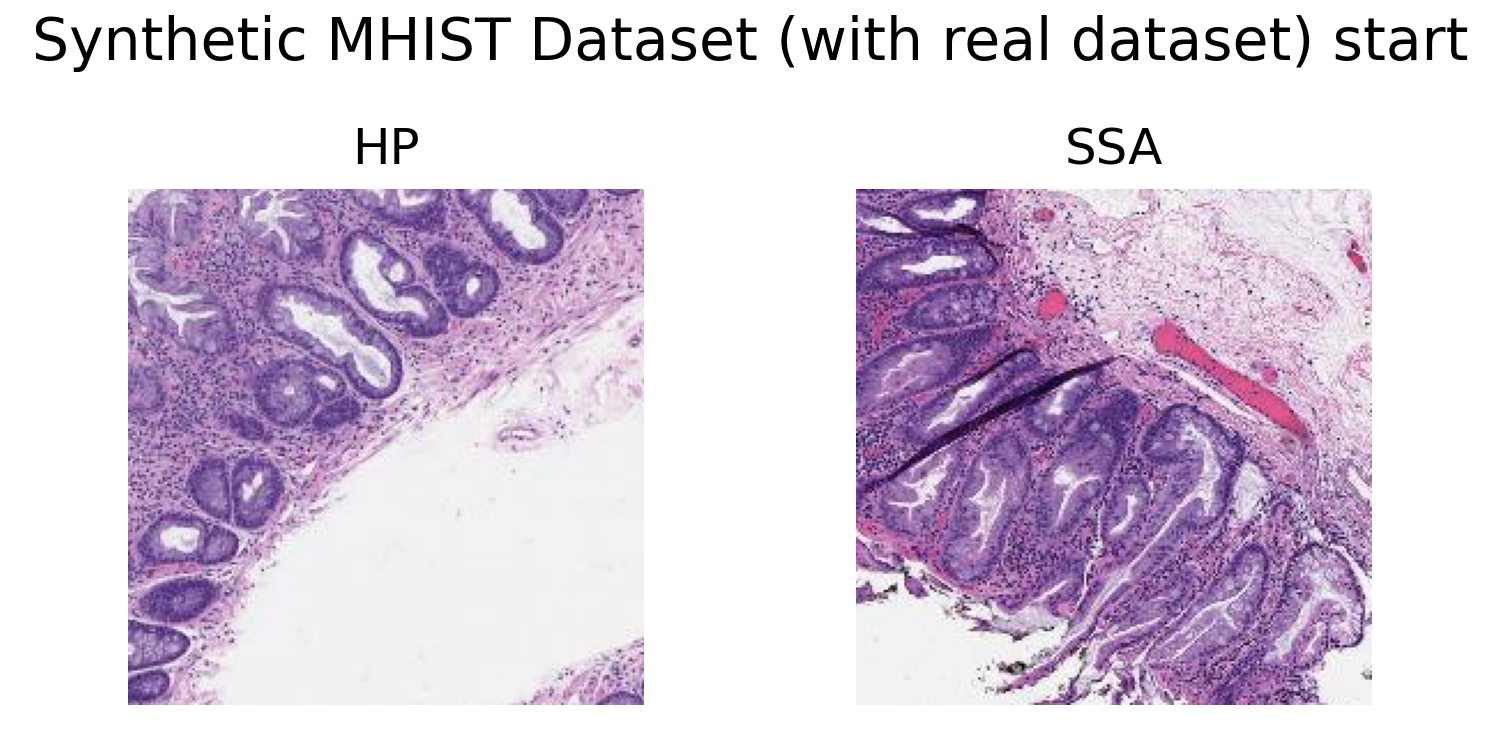
\includegraphics[width=0.48\textwidth]{mhist_real_sample.png}
	\caption{Sample of Synthetic MHIST Dataset created from real images (starting image)}
	\label{fig:mhist_real_sample}
\end{figure}
\begin{figure}[H]
	\centering
	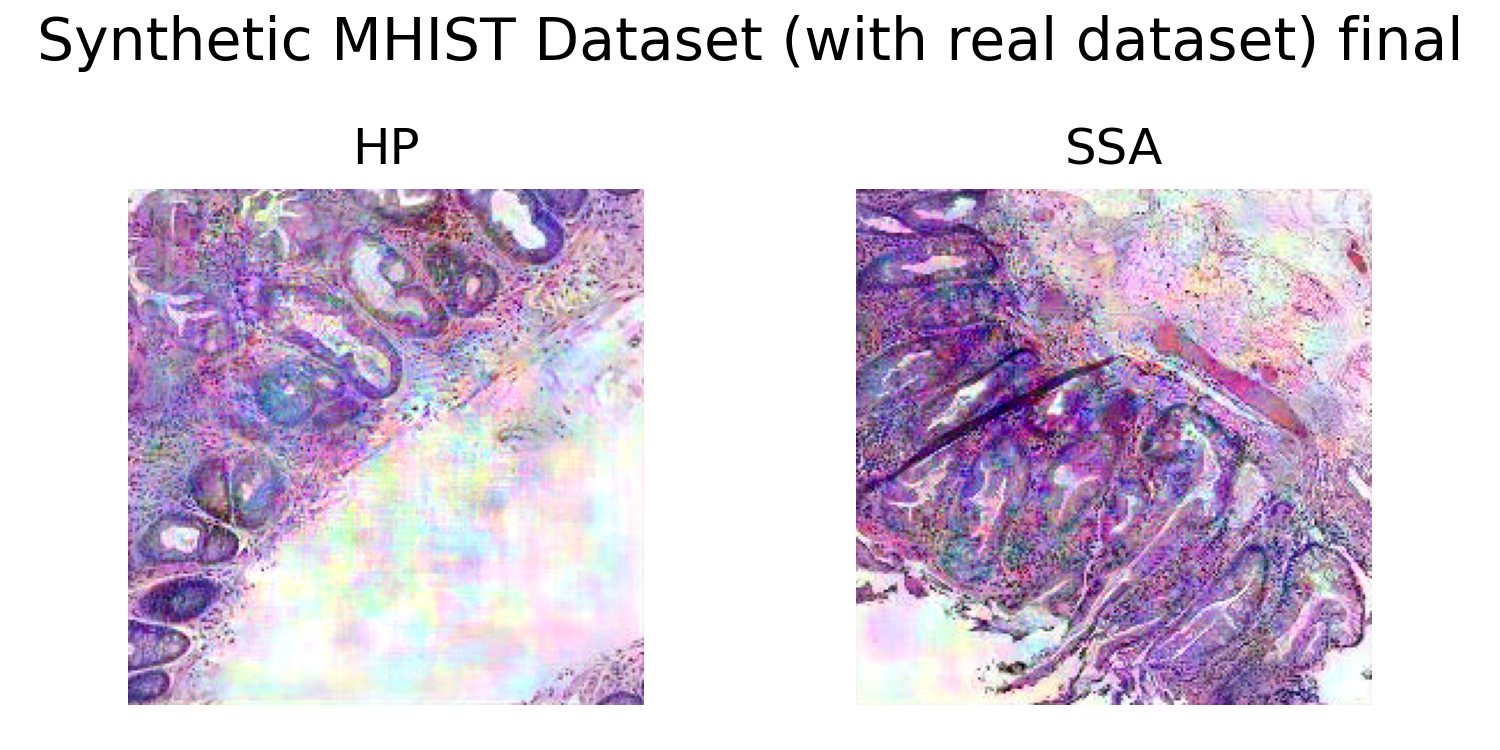
\includegraphics[width=0.48\textwidth]{mhist_real_syn.png}
	\caption{Sample of Synthetic MHIST Dataset created from real images (final image)}
	\label{fig:mhist_real_final}
\end{figure}


\begin{figure}[H]
	\centering
	\includegraphics[width=0.48\textwidth]{mhist_real_syn_hp.png}
	\caption{Synthetic MHIST Dataset created from real images [HP]}
	\label{fig:mhist_real_syn_hp}
\end{figure}

\begin{figure}[H]
	\centering
	\includegraphics[width=0.48\textwidth]{mhist_real_syn_ssa.png}
	\caption{Synthetic MHIST Dataset created from real images [SSA]}
	\label{fig:mhist_real_syn_ssa}
\end{figure}

\subsubsection{Synthetic Dataset using Gaussian noise}
\begin{figure}[H]
	\centering
	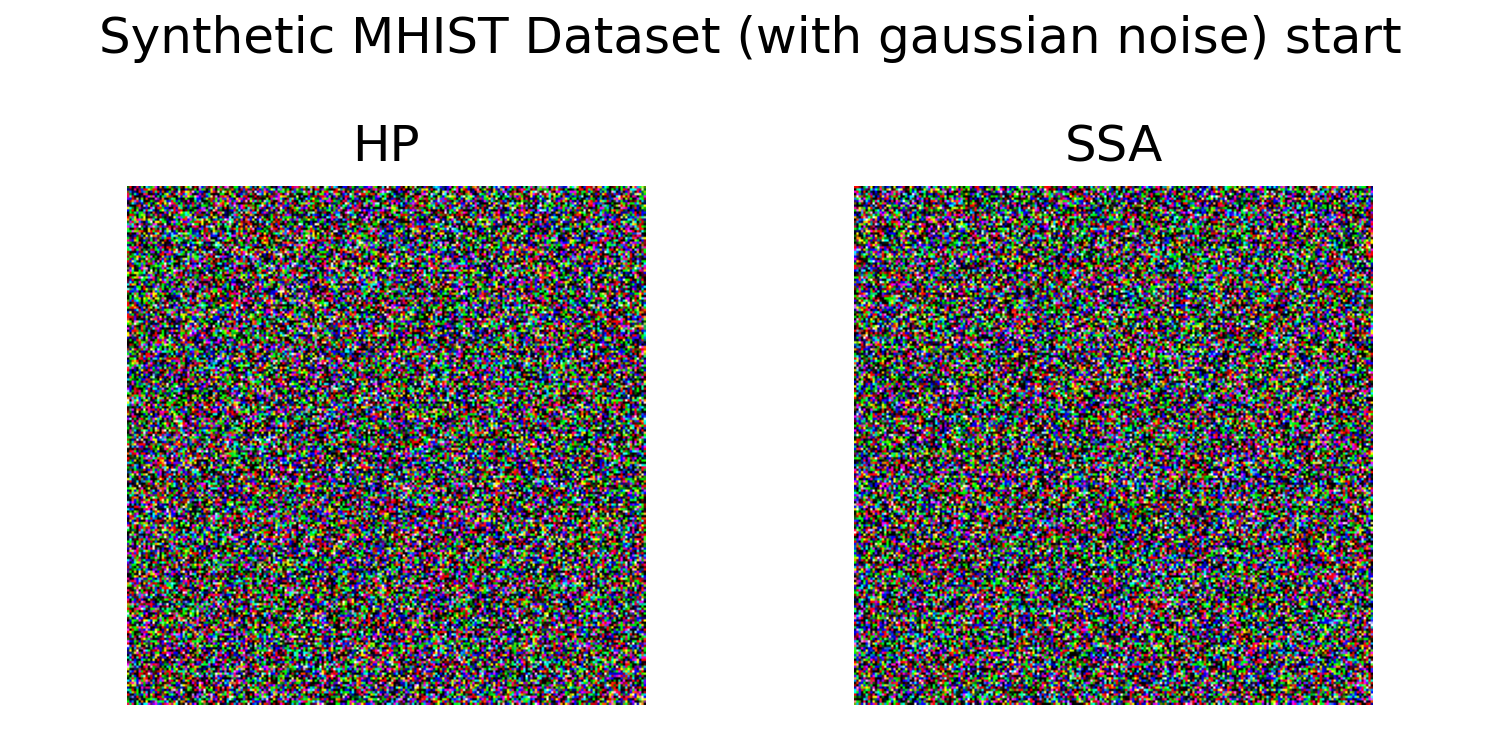
\includegraphics[width=0.48\textwidth]{mhist_noise_sample.png}
	\caption{Sample of Synthetic MHIST Dataset created from Gaussian noise (starting image)}
	\label{fig:mhist_noise_sample}
\end{figure}
\begin{figure}[H]
	\centering
	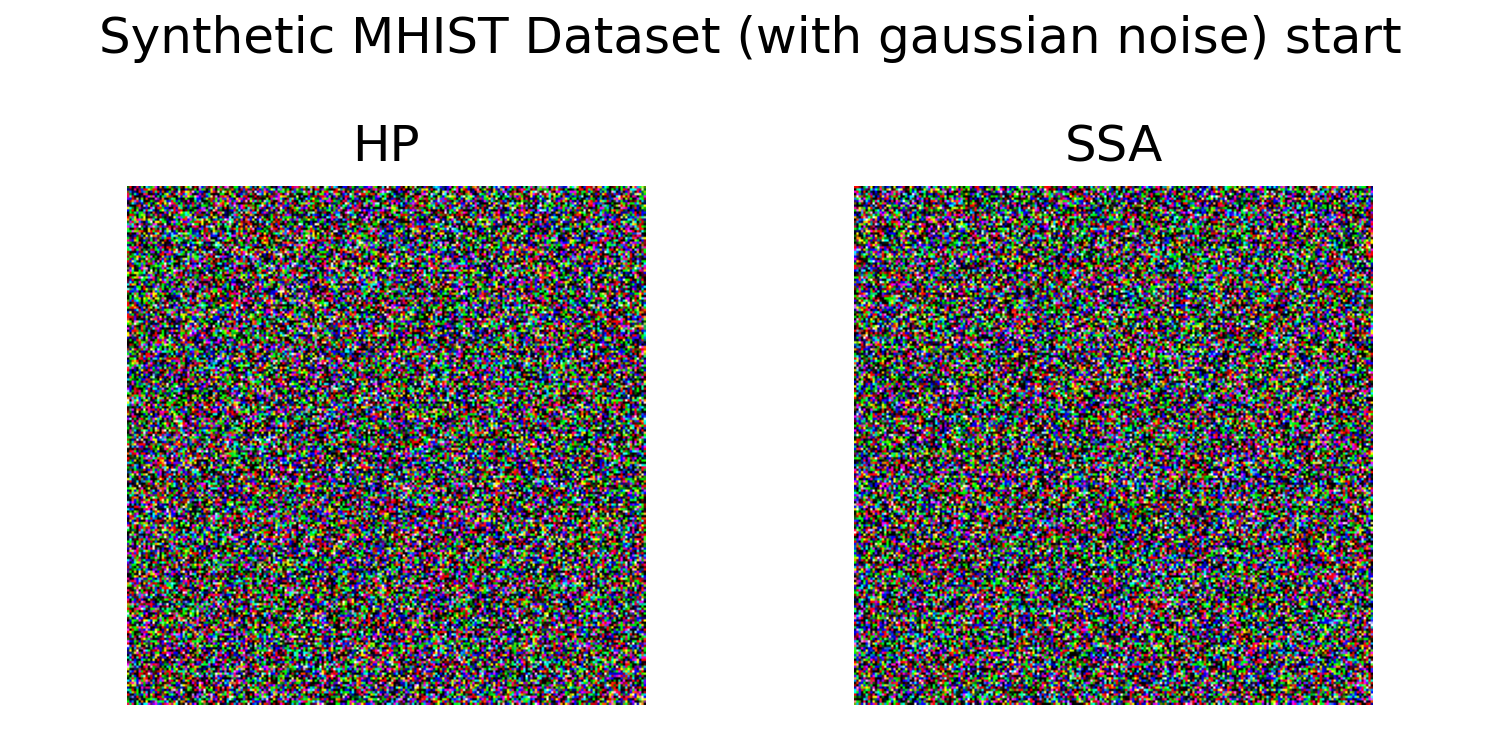
\includegraphics[width=0.48\textwidth]{mhist_noise_sample.png}
	\caption{Sample of Synthetic MHIST Dataset created from Gaussian noise(final image)}
	\label{fig:mhist_noise_final}
\end{figure}


\begin{figure}[H]
	\centering
	\includegraphics[width=0.48\textwidth]{mhist_noise_syn_all.png}
	\caption{Synthetic MHIST Dataset created from Gaussian noise}
	\label{fig:mhist_noise_syn_all}
\end{figure}

\subsubsection{ConvNet-7 using Synthetic Dataset}
\begin{figure}[H]
	\centering
	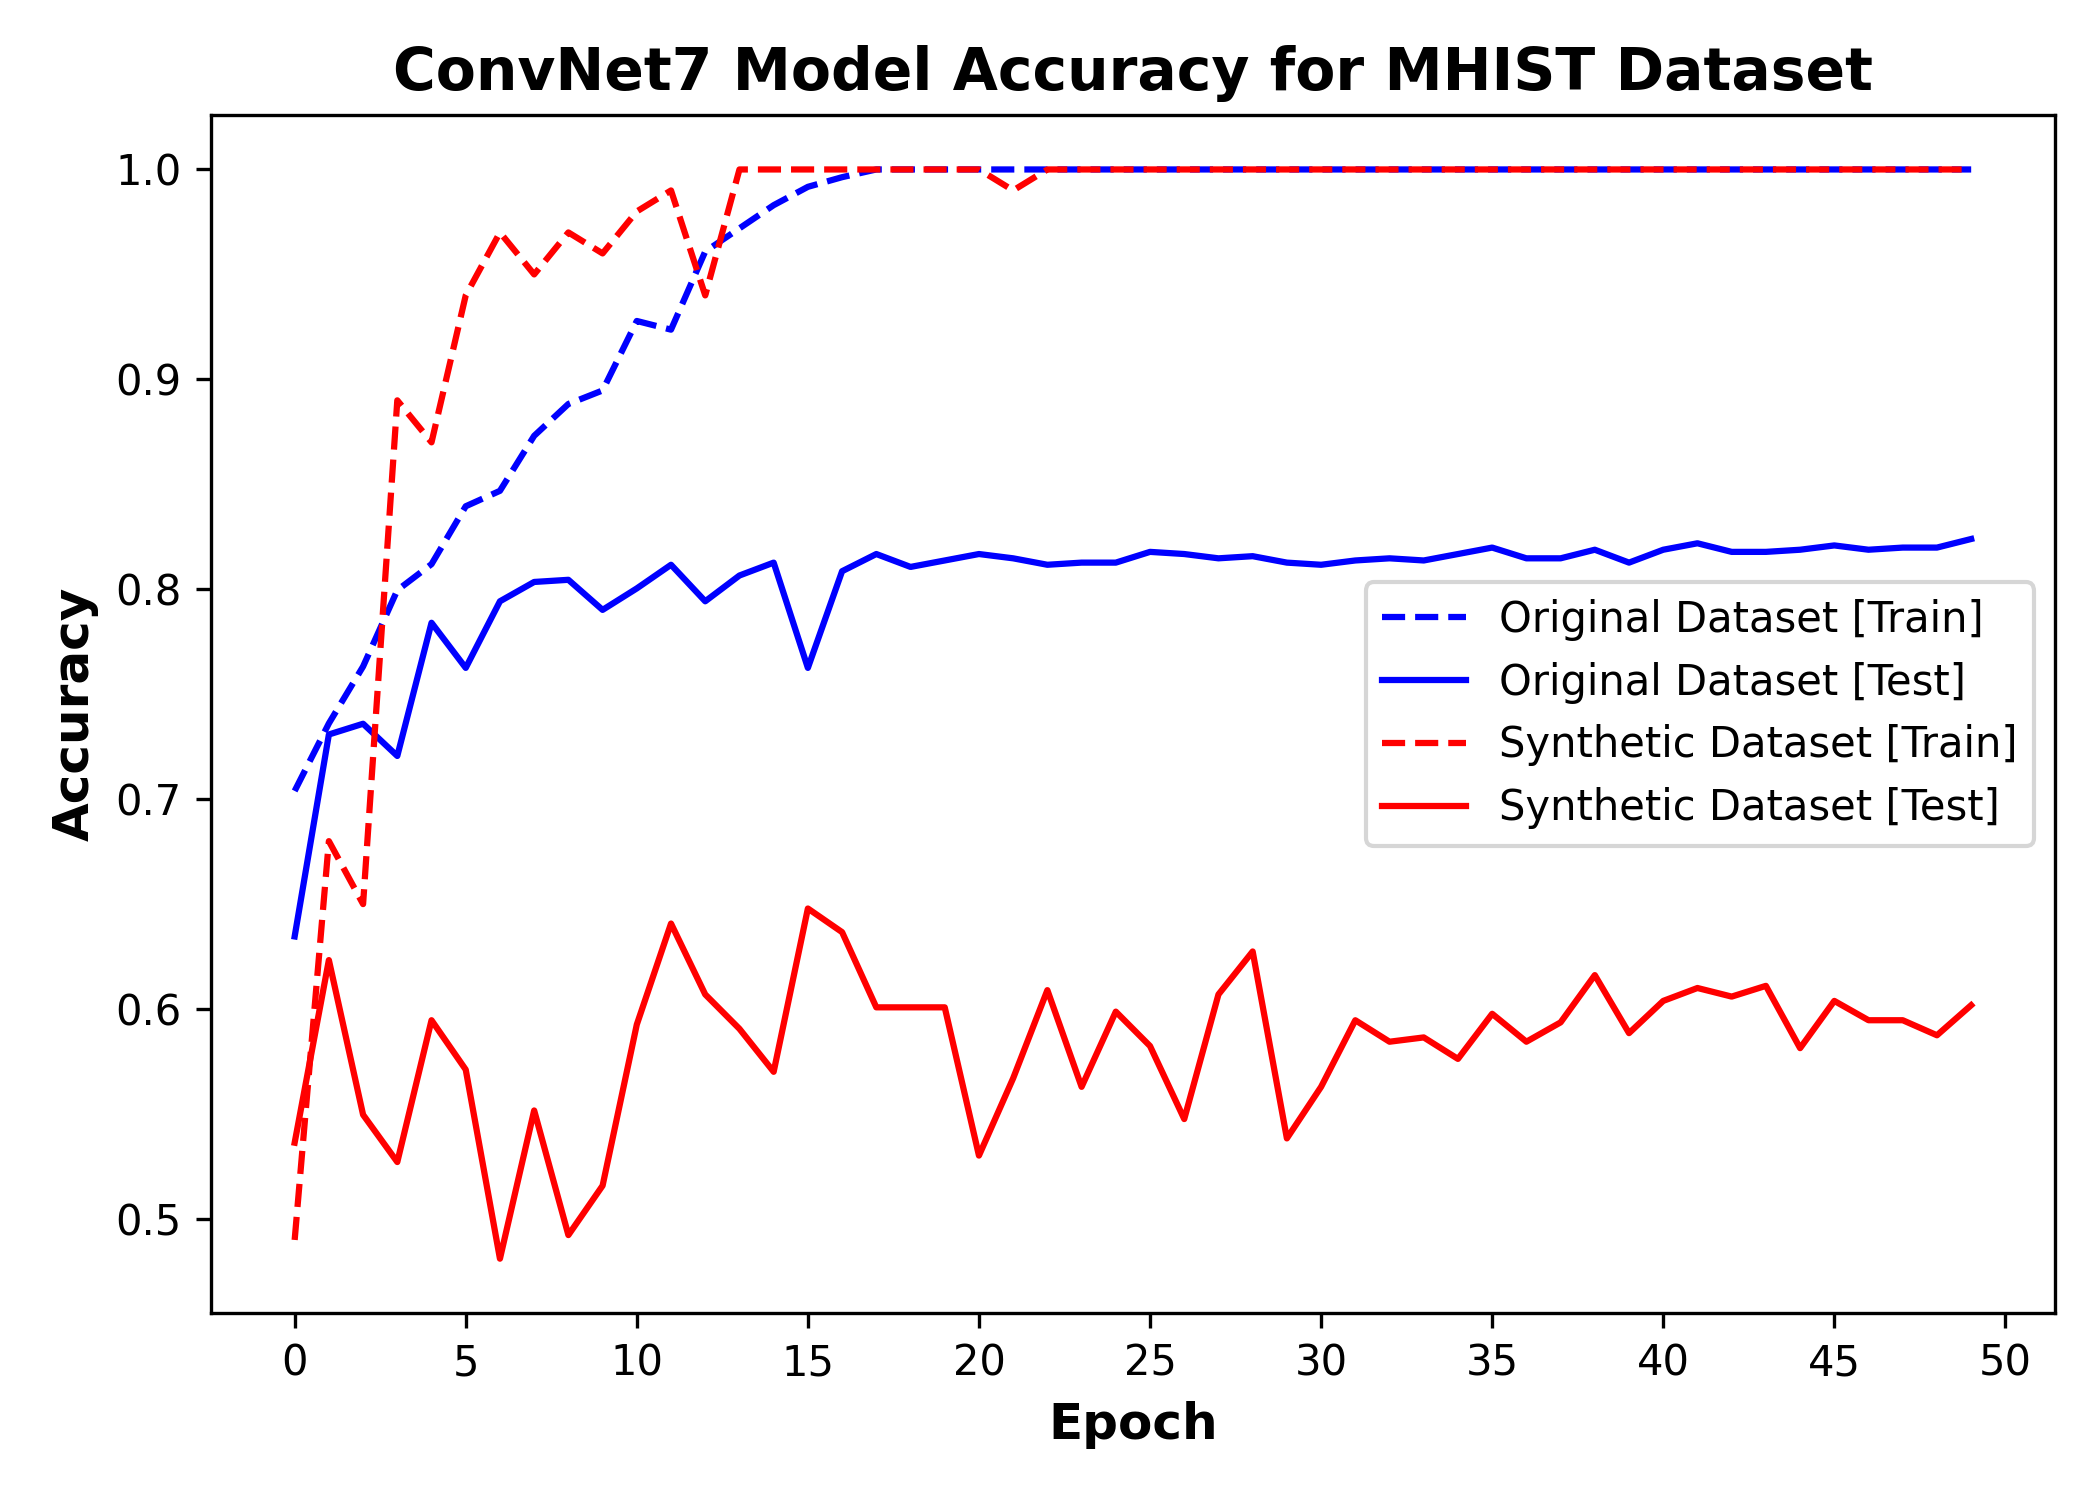
\includegraphics[width=0.48\textwidth]{mhist_syn_acc.png}
	\caption{ConvNet-7 Model Trained using Original and Synthetic dataset}
	\label{fig:mhist_syn_acc}
\end{figure}
\subsubsection{Cross-architecture Generalization - ResNet-18}
\begin{figure}[H]
	\centering
	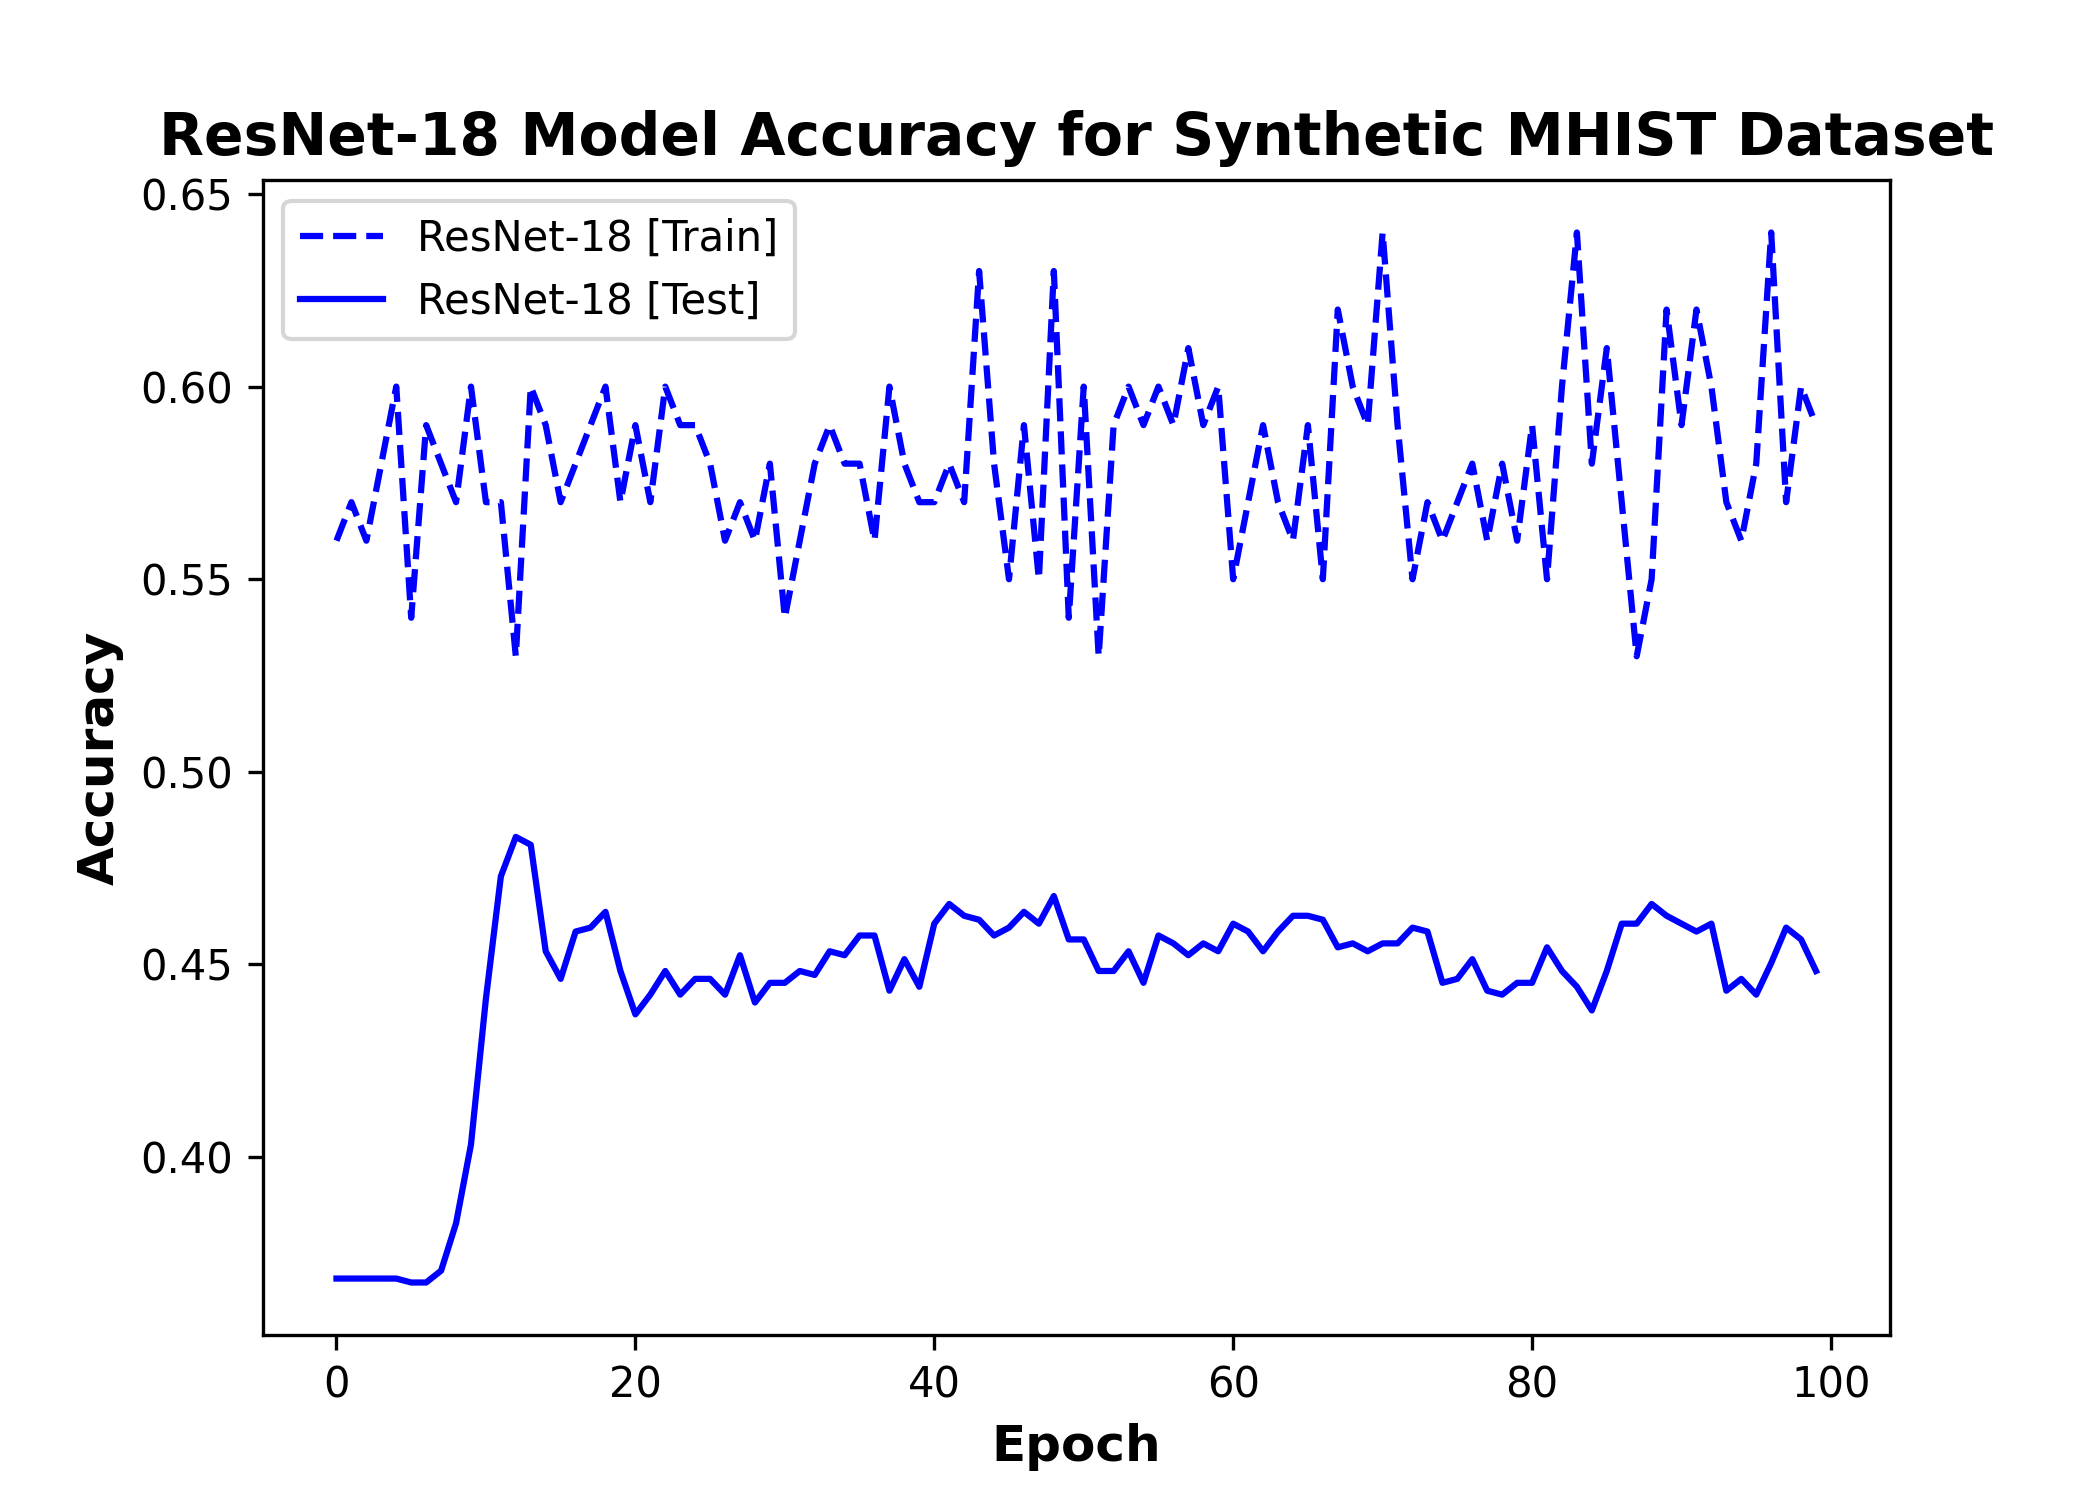
\includegraphics[width=0.48\textwidth]{mhist_resnet_acc.png}
	\caption{ResNet-18 Model Trained using Synthetic dataset}
	\label{fig:mhist_resnet_acc}
\end{figure}

\subsection{Data Distillation Application}
NAS with original dataset took 1607.3 seconds.
with synthetic dataset took 2.8 seconds.

\begin{figure}[H]
	\centering
	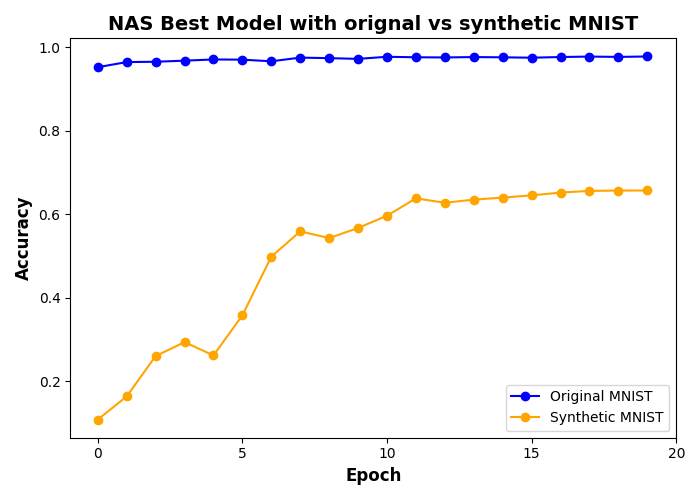
\includegraphics[width=0.48\textwidth]{nas_comparision.png}
	\caption{NAS best model with original vs synthetic MNIST dataset}
	\label{fig:nas_comparision}
\end{figure}

\section{Prioritize Alignment in Dataset Distillation}

\begin{figure}[H]
	\centering
	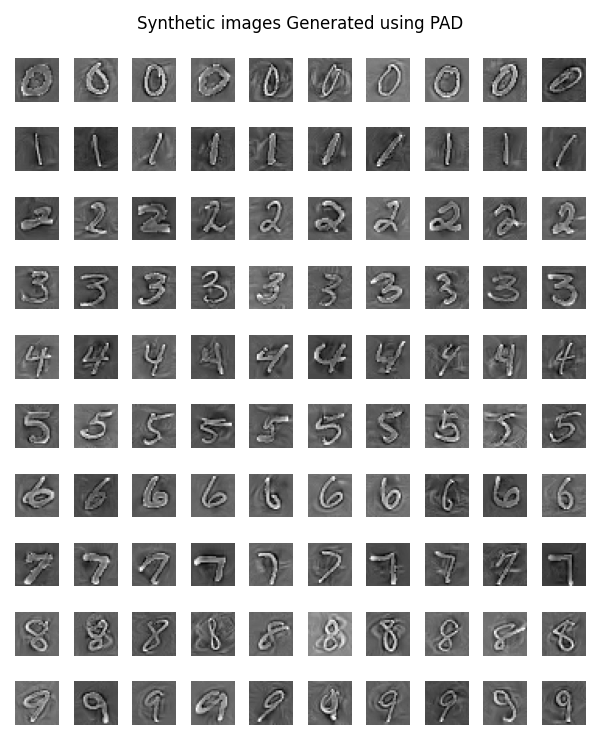
\includegraphics[width=0.48\textwidth]{synthetic_images_task2.png}
	\caption{Synthetic MNIST Dataset using PAD\cite{li2024prioritizealignmentdatasetdistillation}}
	\label{fig:synthetic_images_task2}
\end{figure}

\begin{figure}[H]
	\centering
	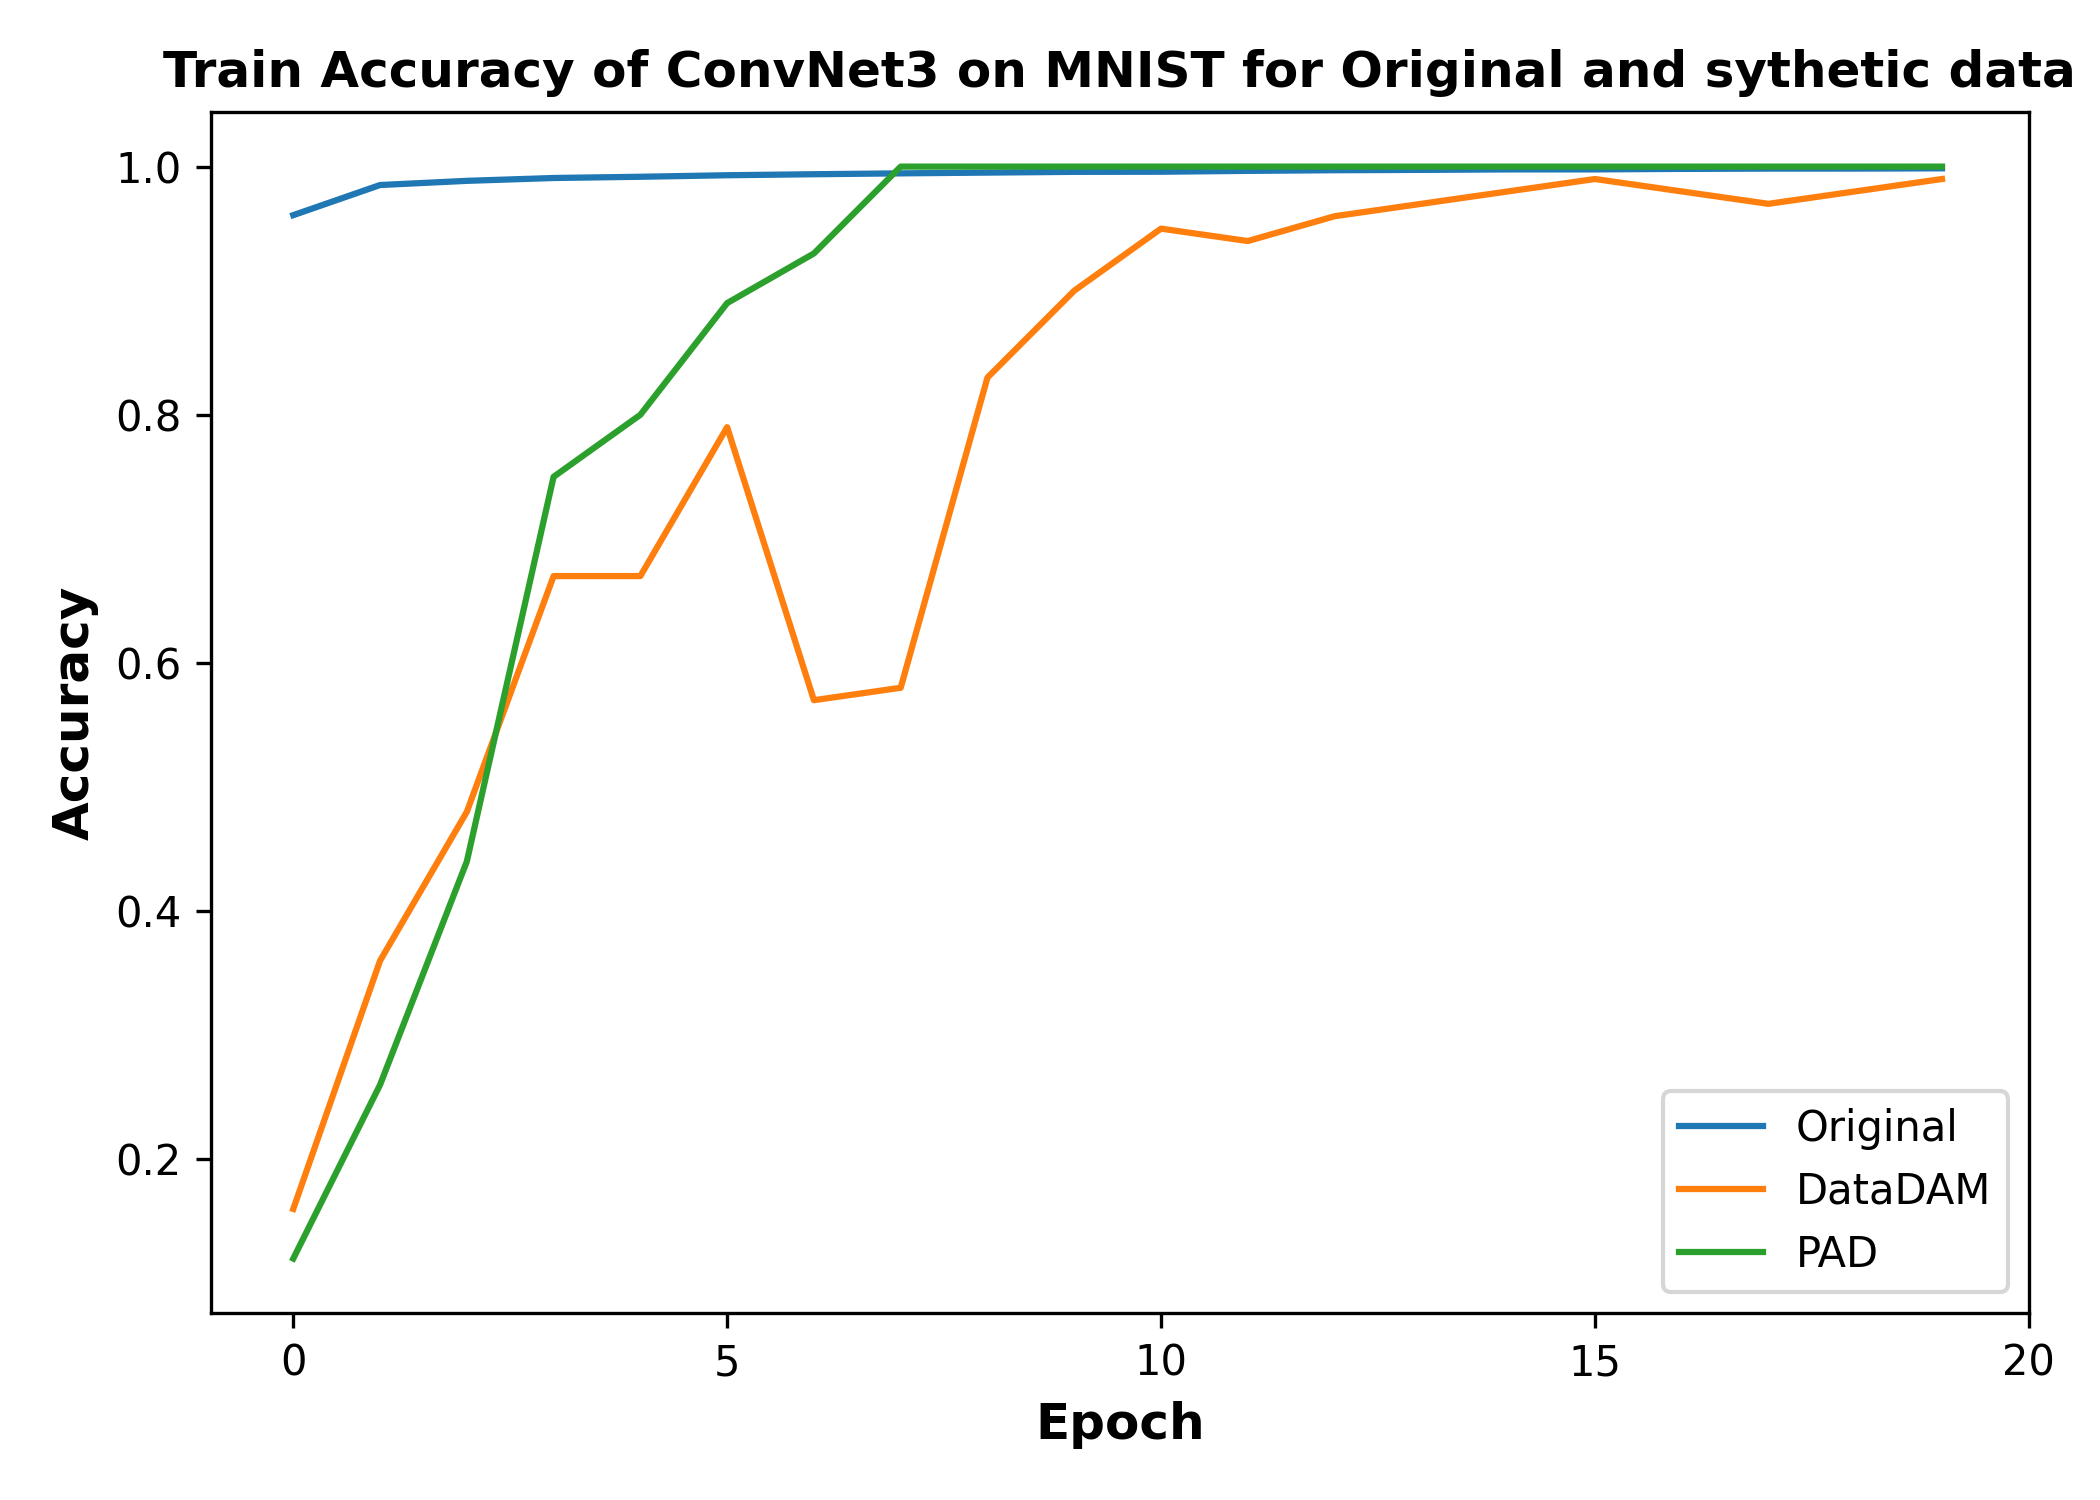
\includegraphics[width=0.48\textwidth]{train_acc_task2.png}
	\caption{}
	\label{fig:train_acc_task2}
\end{figure}

\begin{figure}[H]
	\centering
	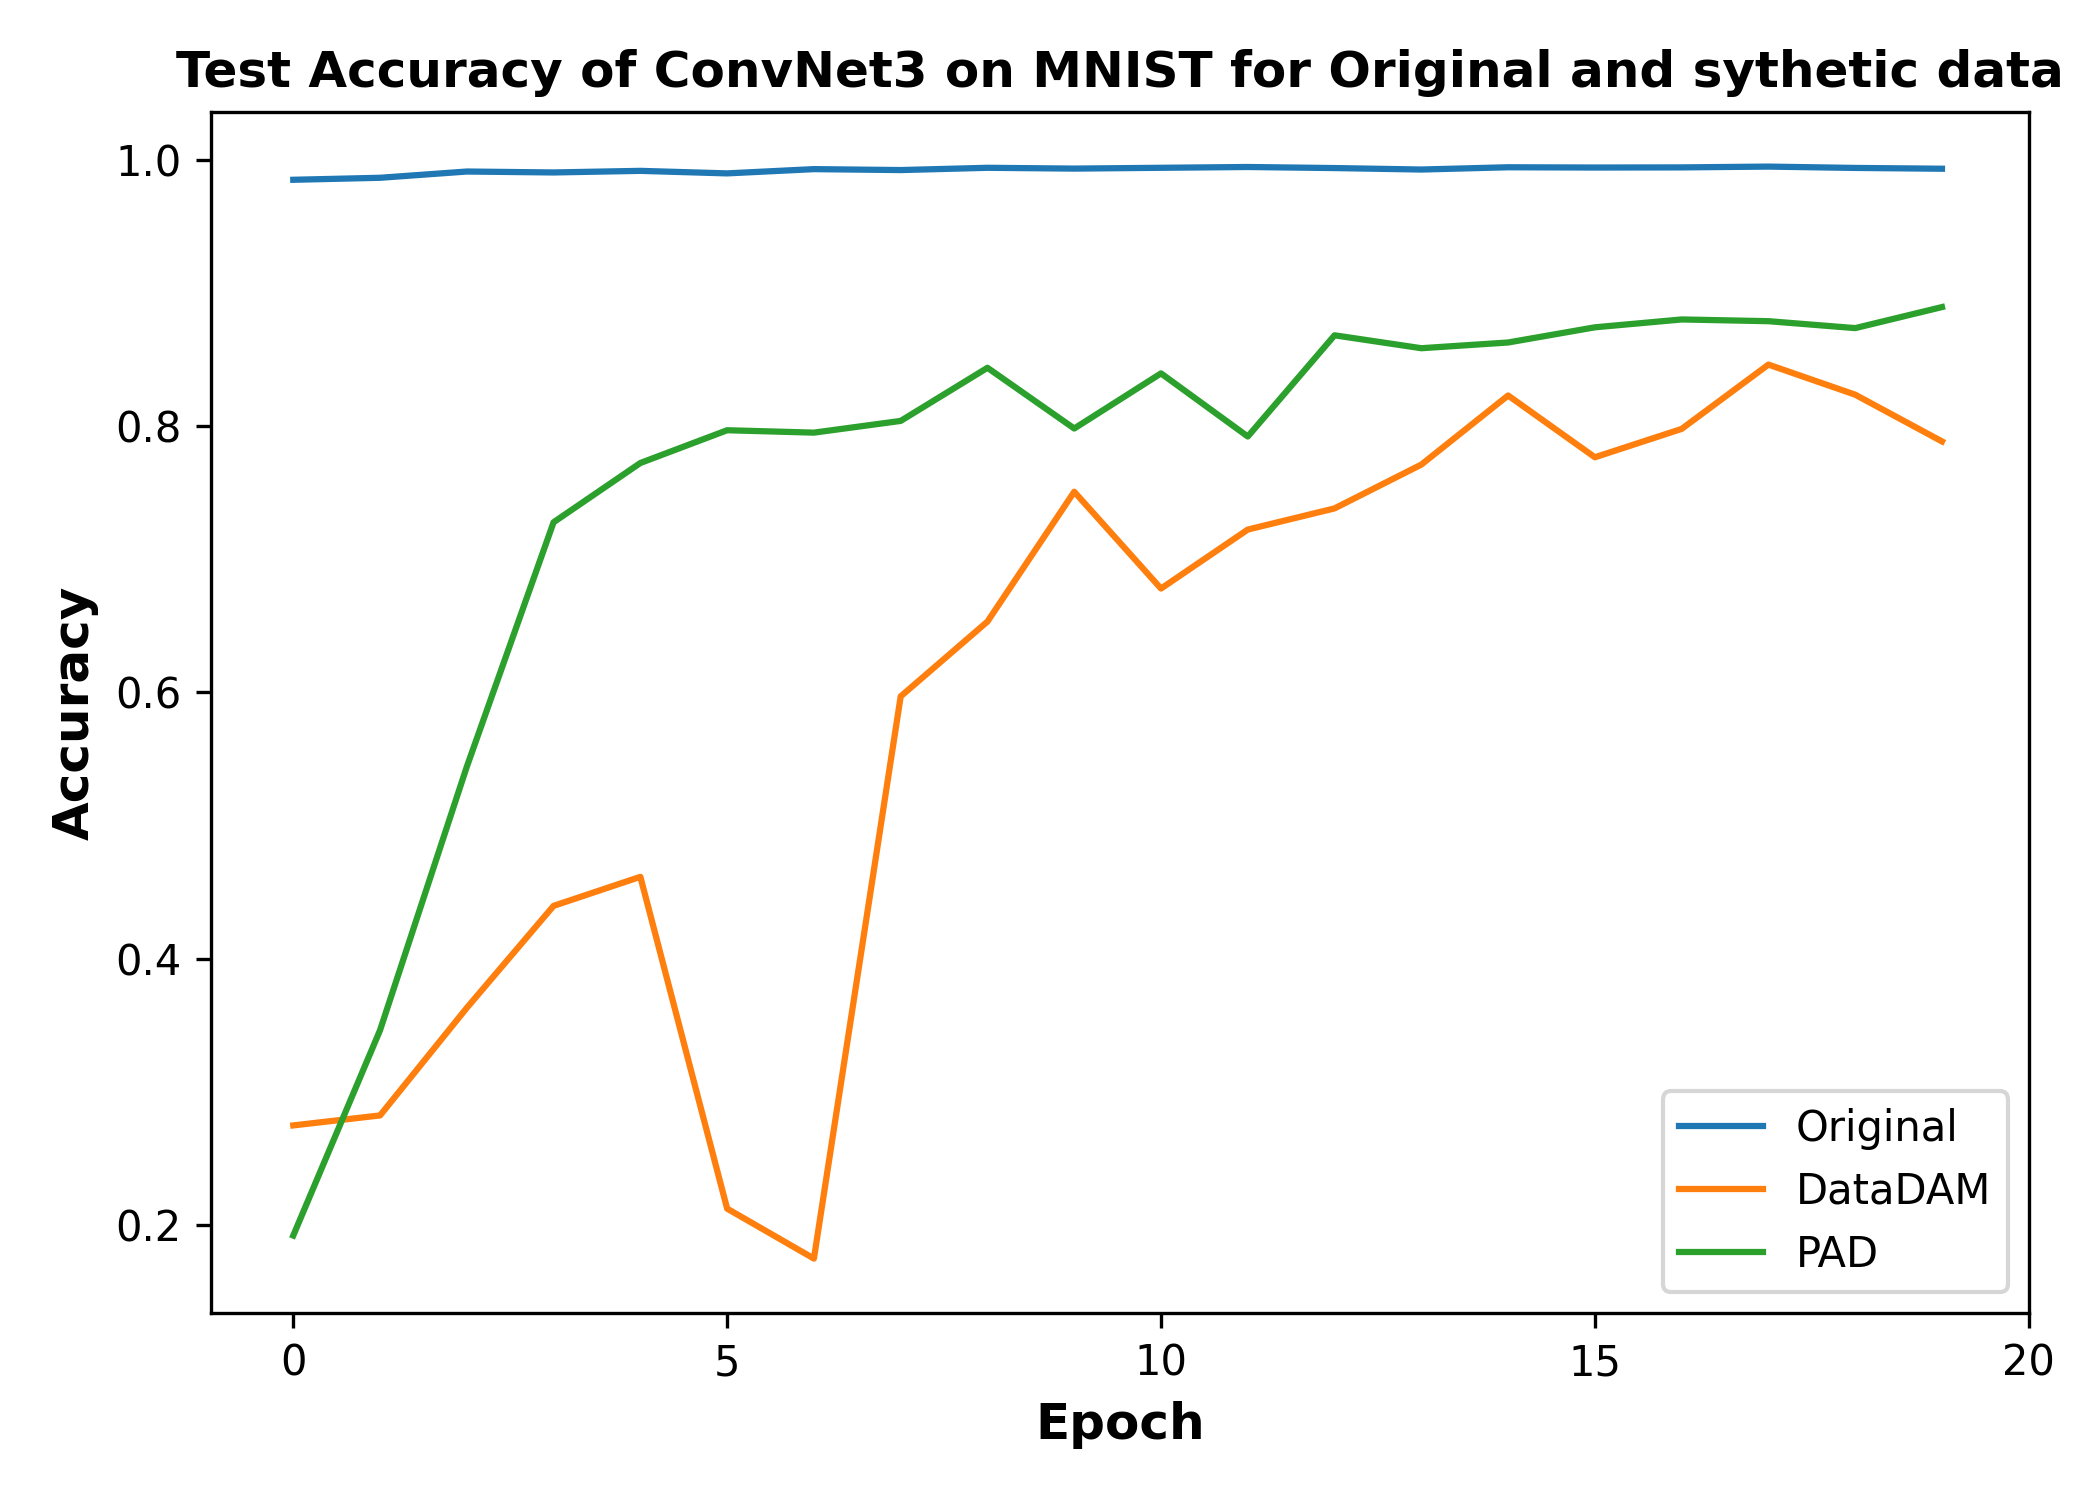
\includegraphics[width=0.48\textwidth]{test_acc_task2.png}
	\caption{}
	\label{fig:test_acc_task2}
\end{figure}

\section{Conclusion}

\section{References}
\nocite{*}
\printbibliography

\end{document}